%% =============================================================================
%% Federated Optimisation on DermaMNIST -- final report (flat Overleaf bundle)
%% Compile with pdfLaTeX + BibTeX. references.bib and all figure PDFs sit next
%% to this file (\graphicspath{{./}}).
%% =============================================================================

\documentclass[11pt,a4paper]{report}

\usepackage[utf8]{inputenc}
\usepackage[T1]{fontenc}
\usepackage{graphicx}
\usepackage{float}   % provides [H] specifier for exact float placement (forces "here, no floating")
\graphicspath{{./}}  % flat Overleaf bundle: all figures sit next to main.tex
\usepackage{booktabs}
\usepackage{amsmath, amssymb}
\usepackage{bm}
\usepackage{microtype}
\usepackage{hyperref}
\usepackage{caption}
\usepackage{xcolor}
\usepackage[margin=2.5cm]{geometry}
\usepackage{setspace}
\usepackage[round,authoryear]{natbib}
\usepackage{titlesec}
\usepackage{fancyhdr}
\onehalfspacing

%% --- Page layout: compact chapter headings + running headers (exemplar style)
% Compact numbered chapter title "1  Introduction" at the top of the page
% (no "Chapter" prefix and no deep vertical drop), as in the example report.
\titleformat{\chapter}[hang]
  {\normalfont\huge\bfseries}{\thechapter}{1em}{}
\titlespacing*{\chapter}{0pt}{0pt}{18pt}

% Running header: chapter (left) and current section (right) in small caps,
% with a rule beneath; page number centred in the footer.
\setlength{\headheight}{14pt}
\renewcommand{\chaptermark}[1]{\markboth{\thechapter.\ #1}{}}
\renewcommand{\sectionmark}[1]{\markright{\thesection.\ #1}}
\fancypagestyle{fancy}{%
  \fancyhf{}%
  \fancyhead[L]{\nouppercase{\scshape\leftmark}}%
  \fancyhead[R]{\nouppercase{\scshape\rightmark}}%
  \fancyfoot[C]{\thepage}%
  \renewcommand{\headrulewidth}{0.4pt}%
  \renewcommand{\footrulewidth}{0pt}%
}

\title{Preserving Rare-Class Signal in Federated Learning\\
\large under Statistical and System Heterogeneity}
\author{Barbara Koch}
\date{}

\begin{document}

%% =============================================================================
%% FRONT MATTER
%% =============================================================================

%% --- Title page (styled after the course exemplar) -------------------------
%% Logo files in this bundle: cam_logo_trim.png (University of Cambridge),
%% dis_logo.png (DiS MPhil programme), college_crest.png (college crest).
%% Each \coverlogo slot falls back to a labelled placeholder box if its file
%% is missing.
\newcommand{\coverlogo}[3]{% #1 = filename, #2 = height, #3 = placeholder label
  \IfFileExists{#1}{\includegraphics[height=#2]{#1}}%
    {\fbox{\parbox[c][#2][c]{0.34\textwidth}{\centering\scriptsize\itshape #3}}}}
\begin{titlepage}
\centering

% institutional logos: Cambridge (left), DiS MPhil (right)
% top-aligned and flush to the top of the page, as in the example report
\vspace*{-1.2cm}
\noindent\makebox[\textwidth]{%
  \raisebox{-\height}{\coverlogo{cam_logo_trim.png}{1.5cm}{University of Cambridge logo}}\hfill
  \raisebox{-\height}{\coverlogo{dis_logo.png}{1.5cm}{DiS MPhil logo}}}

\vspace*{\fill}

{\huge\bfseries
 \setstretch{1.1}
 Preserving Rare-Class Signal in\\
 Federated Learning\par}
\vspace{0.9em}
{\large\bfseries under Statistical and System Heterogeneity\par}

\vspace{2.8em}
{\large\scshape\bfseries A Report Presented\par}
\vspace{0.45em}
{\scshape\bfseries by\par}
\vspace{0.45em}
{\Large\scshape\bfseries Barbara Koch\par}

\vspace{2.6em}
{\bfseries Departments}\par
\vspace{0.4em}
{\bfseries Department of Applied Mathematics and Theoretical Physics\par}
{\bfseries Department of Physics (Cavendish Laboratory)\par}

\vspace{1.4em}
{\bfseries Degree}\par
\vspace{0.4em}
{\bfseries MPhil in Data Intensive Science\par}

\vspace{1.4em}
{\bfseries Supervision}\par
\vspace{0.4em}
{\bfseries Dr Joshua Kaggie\par}

\vspace*{\fill}

% college crest above the college / university / date block
\coverlogo{peterhouse_crest.png}{2.2cm}{Peterhouse crest}\par
\vspace{0.6em}
{\large\scshape\bfseries Peterhouse\par}
{\large\scshape\bfseries University of Cambridge\par}
{\large\scshape\bfseries 1st July 2026\par}
\end{titlepage}

% front matter: page number only, no running header
\pagestyle{plain}

\begin{abstract}
Federated learning lets institutions train a shared model without pooling private
data, but real federations are heterogeneous in both their data and their compute,
and medical image datasets are severely class-imbalanced. This thesis studies
federated optimisation on DermaMNIST, a seven-class dermatology benchmark
dominated by a single benign class, comparing FedAvg, FedProx, and FedNova across
controlled statistical- and system-heterogeneity regimes and reporting test
macro-F1 at the best-validation checkpoint. Rather than crowning a universal
winner, it maps the regimes in which each method preserves or loses rare-class
signal. The central finding is that under Li-style straggler asymmetry the FedProx
advantage (about $+0.115$ macro-F1) is carried almost entirely by its
$\gamma$-inexact acceptance of partial updates rather than by the proximal term,
and that FedNova is robust under deterministic learning-rate asymmetry yet
collapses under random per-round stragglers. Across the failing regimes, rare
lesions are misrouted into the majority class. These results come from controlled
DermaMNIST benchmark simulations with $n=3$ mechanism probes, and map regimes
rather than establishing a universal optimiser ranking.
\end{abstract}

\chapter*{Declaration}
\addcontentsline{toc}{chapter}{Declaration}
This thesis contains 6,784 words.

I declare that this thesis is original and is submitted as part of the requirements
for the degree. Except where explicitly stated, it contains nothing which is the
outcome of work done in collaboration with others.

I used GitHub for version control and repository management. Claude by Anthropic
was used for assistance with coding and debugging, and ChatGPT by OpenAI was used
for organisation, planning, and structuring support. The experiments, analysis,
interpretation, and final submitted text remain my own responsibility.

\tableofcontents
\listoffigures
\listoftables


%% =============================================================================
%% CHAPTER 1: INTRODUCTION
%% =============================================================================
% body: running headers (chapter left, section right) from here on
\pagestyle{fancy}
\chapter{Introduction}
\label{ch:intro}

\section{Motivation}
\label{sec:intro-motivation}

Diagnostic models improve with large, diverse image collections, but in medicine
those collections are fragmented across institutions and cannot usually be pooled
centrally because of privacy regulation and governance. Federated learning
sidesteps this by keeping each institution's data in place and exchanging only
model updates \citep{mcmahan2017fedavg, rieke2020future, sheller2020medicalfl},
which makes it a natural setting for collaborative learning across hospitals
\citep{kairouz2021advances, pati2022fets}. It also introduces two difficulties
that are acute in medicine. Under \emph{statistical heterogeneity}, sites see
different case mixes, so client data is non-IID \citep{zhao2018noniid}; under
\emph{system heterogeneity}, sites differ
in compute and availability, so some clients return only partial updates in a
round. The two coincide most damagingly when the under-resourced site is also the
one holding the rare cases.

Medical data is, in addition, severely class-imbalanced, a recognised obstacle
for federated training \citep{wang2021classimbalance}. DermaMNIST
\citep{yang2023medmnistv2}, derived from the HAM10000 dermatoscopic collection
\citep{tschandl2018ham10000} and used throughout this thesis, is dominated by
benign melanocytic nevi, while the diagnostically urgent lesions are rare;
federated learning has itself been applied to skin-lesion classification
\citep{yaqoob2023skinfl}. A model
can therefore post high accuracy while failing on exactly the lesions that matter,
so we report macro-F1 and per-class rare-class diagnostics rather than accuracy.
Crucially, the information needed to recognise a rare lesion reaches the global
model only through the updates of the client that holds it; if heterogeneity
under-weights or discards those updates, the rare-class signal is lost. The
quantity that governs rare-class performance is thus the \emph{flow of
rare-client signal into the global model}, and the federated optimiser --- not the
network architecture --- is the lever that protects or forfeits it.

\section{Research problem}
\label{sec:intro-problem}

The optimisers proposed for these conditions --- FedAvg \citep{mcmahan2017fedavg},
FedProx with its proximal term and tolerance for inexact updates
\citep{li2020fedprox}, and FedNova with its work-normalised aggregation
\citep{wang2020fednova} --- are usually compared by which scores higher on a task
\citep{li2022niidbench}, rarely isolating \emph{why}, often conflating the two
heterogeneities, and judging by accuracy. This thesis instead asks \emph{when}
each method preserves rare-class performance, treating the answer as a
\emph{regime map} rather than a universal ranking. It separates four levers that
are usually bundled together --- the data partition, the optimiser, the
partial-update protocol, and loss-side imbalance correction --- and varies them one
at a time. All experiments are simulated federated learning on a controlled
benchmark, so the work maps mechanisms rather than validating a clinical
deployment.

\section{Research questions and contributions}
\label{sec:intro-questions}

This framing raises four questions. Because the literature often credits FedProx
and FedNova with broad gains, the thesis first asks whether statistical
heterogeneity alone is enough to separate FedAvg and FedProx or whether additional
stress is required; then, where FedProx does help under stragglers, whether that
benefit comes from its proximal regularisation or from its $\gamma$-inexact
acceptance of partial updates; whether FedNova's work-normalisation is robust in
general or only under deterministic learning-rate asymmetry, failing under random
round-to-round straggling; and finally whether rare-class collapse into the
majority class is the shared failure mode, and whether the FedProx advantage is
merely class-imbalance correction in disguise. Chapter~\ref{ch:results} follows
this order: statistical heterogeneity (\S\ref{sec:statistical-heterogeneity}), the
proximal coefficient (\S\ref{sec:mu-sensitivity}), straggler asymmetry
(\S\ref{sec:li-straggler}), FedNova regime-dependence (\S\ref{sec:lr-asymmetry}),
and rare-class collapse with the loss-side comparison
(\S\ref{sec:rare-class-collapse}).

Answering these yields the contributions of the thesis. It maps the regimes in
which FedAvg, FedProx, and FedNova preserve or lose rare-class signal, and
decomposes the FedProx straggler-regime advantage into its proximal and
$\gamma$-inexact components using matched class-disjoint (L4) and quantity-only
(L1) partitions that fix when the effect can appear. It then characterises
FedNova's regime-dependence across deterministic and random system heterogeneity,
and identifies rare-class collapse into the dominant melanocytic-nevi class as the
common failure mode. Finally, through the same L4/L1 decomposition, it shows the
FedProx straggler-regime advantage to be a drift-and-protocol effect, with
weighted cross-entropy a competitive loss-side alternative rather than evidence
that the advantage is merely class-imbalance correction in disguise.


%% =============================================================================
%% CHAPTER 4: METHODS
%% =============================================================================
\chapter{Methods}
\label{ch:methods}

\section{Problem setup and design}
\label{sec:method-problem}
\label{sec:method-rationale}

We consider a federation of $K$ clients coordinated by a central server that
together train a single global model without exchanging raw data
(Figure~\ref{fig:fl-workflow}). Client $i$ holds a private training set $D_i$ of
$n_i$ examples, with $N = \sum_i n_i$. In each round $t$ the server broadcasts the
global model $w^{t}$; every participating client runs $E$ epochs of local SGD on
$D_i$ to obtain $w_i^{t+1}$ and returns its update
\[
  d_i = w_i^{t+1} - w^{t}.
\]
The baseline rule, FedAvg \citep{mcmahan2017fedavg}, recombines these by the
sample-weighted mean
\[
  w^{t+1} = \sum_i \frac{n_i}{N}\, w_i^{t+1}.
\]
FedProx \citep{li2020fedprox} and FedNova \citep{wang2020fednova} modify,
respectively, the local objective and the way the updates $d_i$ are normalised
before combination (\S\ref{sec:method-optimisers}).

\begin{figure}[t]
\centering

\includegraphics[width=0.70\textwidth]{F_federated_learning_workflow.pdf}
\caption{Federated learning loop (conceptual; \emph{simulated} on a single
machine in this thesis). Each round the server broadcasts the global model
$w^{t}$, clients train locally on private data $D_i$ and return model updates
$d_i$ (not raw data), and the server aggregates them into $w^{t+1}$; the loop
repeats for $R$ rounds.}
\label{fig:fl-workflow}
\end{figure}

The aim is not to crown a universal winner among the three optimisers but to map
which regimes preserve or lose rare-class performance. The design separates three
axes the FL literature often conflates.
\emph{Statistical heterogeneity} controls which clients own the rare-class signal
--- from IID, through Dirichlet label skew \citep{hsu2019dirichlet}, to
class-disjoint clients --- and is fixed before training by the data partition; it
determines \emph{where} rare-class information resides. \emph{System
heterogeneity} controls whether that signal reaches aggregation: a straggler
completes fewer local steps, and its partial update may be dropped or accepted, or
it may take smaller steps under a lower learning rate. \emph{Optimiser and
protocol choices} then determine the global response. The two heterogeneities
interact most sharply when the client carrying the rare classes is also the one
that is slow or under-weighted.

This motivates the concept that organises the thesis, \emph{rare-client signal
flow}: the per-round contribution that the rare-class-holding client makes to the
global update. A rare class is learned only to the extent that the information in
that client's update $d_i$ reaches and persists in $w^{t+1}$, so the organising
hypothesis is that rare-class performance is preserved precisely when rare-client
signal continues to reach the global model. The matched two-client partitions L4
(class-disjoint) and L1 (quantity-only control) isolate this
(\S\ref{sec:method-partitions}). Performance is measured throughout by test
macro-F1 at the best-validation checkpoint (\S\ref{sec:method-metrics}).

The optimiser set is deliberately limited rather than exhaustive, and the
four-condition decomposition lacks a FedAvg $+$ $\gamma$-inexact cell, so its
rescue attribution is to the \emph{FedProx $+$ $\gamma$-inexact protocol}, not to
$\gamma$-inexact acceptance alone.

\section{Dataset, metrics, and reporting}
\label{sec:method-dataset}
\label{sec:method-metrics}

All experiments use DermaMNIST from MedMNIST~v2 \citep{yang2023medmnistv2}, a
seven-class dermatology benchmark derived from the HAM10000 dataset of
dermatoscopic skin-lesion images \citep{tschandl2018ham10000}. The task is
single-image classification at $28 \times 28$ RGB resolution. Splits follow the
canonical MedMNIST~v2 release with $7007$ training, $1003$ validation, and $2005$
test images, permuted to channel-first float, scaled to $[0, 1]$, and normalised
with ImageNet channel statistics.

The benchmark is severely class-imbalanced (Figure~\ref{fig:dataset-classes},
Table~\ref{tab:dataset-classes}): mel-nevi dominates the training set, while
dermatofibroma and vascular lesions have so little support that failing to learn
them incurs a large macro-F1 penalty at almost unchanged accuracy. Melanoma is
mid-support but is kept in the canonical rare-class group
$\mathrm{RARE\_IDX} = \{\text{dermato}, \text{melanoma}, \text{vascular}\}$, since
missing a melanoma is the highest-priority failure. Mel-nevi acts as the
\emph{majority attractor}: under failing protocols, rare-class images are routed
into it, so accuracy stays high while macro-F1 collapses. Partitions
(\S\ref{sec:method-partitions}) apply to the training set only; validation and test
sets stay global and class-stratified, so any test-set rare-class collapse is not a
partition artefact.

\begin{table}[H]
\centering
\small
\caption{DermaMNIST class supports and roles in this thesis. Train
prevalence and test support are computed directly from the MedMNIST~v2
release; the train support totals $7007$ and the test support totals
$2005$. The rare-class group $\mathrm{RARE\_IDX} = \{\text{dermato},
\text{melanoma}, \text{vascular}\}$ defines the rare-class F1 used
throughout Chapter~\ref{ch:results}.}
\label{tab:dataset-classes}
\resizebox{\textwidth}{!}{%
\begin{tabular}{l c c p{0.42\linewidth}}
\toprule
Class                              & Train prevalence & Test support & Role in thesis \\
\midrule
mel-nevi (melanocytic nevi)        & $66.9\,\%$       & $1341$       & Majority attractor; collapse-mode prediction class \\
melanoma                           & $11.1\,\%$       & $223$        & Mid-support, high clinical priority; in rare-class group \\
dermatofibroma                     & $1.1\,\%$        & $23$         & Smallest class; in rare-class group \\
vascular lesions                   & $1.4\,\%$        & $29$         & Second smallest; in rare-class group \\
remaining (akiec, bcc, b-kerat)    & $19.4\,\%$       & $389$ total  & Per-class reporting only; no special role \\
\bottomrule
\end{tabular}%
}
\end{table}

\begin{figure}[H]
\centering

\includegraphics[width=0.82\textwidth]{F_dataset_classes.pdf}
\caption{DermaMNIST: one example image per class (top) and training-set class
prevalence (bottom). Melanocytic nevi (nv) dominate at $66.9\,\%$, while the rare
classes used throughout --- dermatofibroma ($1.1\,\%$), vascular ($1.4\,\%$), and
melanoma ($11.1\,\%$; orange) --- are a small fraction of the data. This imbalance
is why raw accuracy is misleading and the thesis ranks optimisers by macro-F1.}
\label{fig:dataset-classes}
\end{figure}

The primary metric throughout is \emph{test macro-F1 at the best-validation
checkpoint}, computed on the global test set: macro-F1 weights all seven classes
equally and is sensitive to rare-class collapse, whereas raw accuracy saturates at
the $\approx 66.9\,\%$ mel-nevi floor. Secondary diagnostics are per-class F1;
per-class recall (the confusion-matrix diagonal $P(\hat{y} = c \mid y = c)$);
rare-class F1 over $\mathrm{RARE\_IDX}$; rare-to-mel-nevi misrouting, the mean over
rare classes of $P(\hat{y} = \text{nv} \mid y = c)$; convergence curves; and
per-client update norms (diagnostic only). Balanced accuracy is stored only as a
sanity check, never used to rank optimisers. Validation macro-F1 selects the best
checkpoint round-by-round; test metrics are evaluated once at that checkpoint.
Evaluation uses argmax predictions. A
\emph{protocol flip} is a sign reversal of $\Delta = \mathrm{FedProx} -
\mathrm{FedAvg}$ between the best-validation, final-round, and last-$K$ summaries,
reported as a robustness check.

Three seed tiers are reported distinctly (Table~\ref{tab:seed-tiers}); sample SDs
use the unbiased ($N-1$) denominator. The \emph{node-pinned L4} configuration is a variance control: it re-runs L4 cells
on a single compute node with matched seeds to isolate cross-node CUDA
non-determinism from any optimiser effect.

\begin{table}[H]
\centering
\small
\caption{Seed-tier reporting protocol. Wins is the number of paired
within-seed comparisons in which FedProx exceeds FedAvg. Wilcoxon refers
to the paired signed-rank test \citep{demsar2006classifier}, used only where
$n = 10$ provides sufficient power.}
\label{tab:seed-tiers}
\begin{tabular}{c p{0.32\linewidth} p{0.36\linewidth}}
\toprule
Tier         & Statistical reporting                                                                            & Use case                                                                                                  \\
\midrule
$n = 10$     & Mean $\pm$ sample SD; paired $\Delta$; wins; paired Wilcoxon signed-rank where meaningful        & Headline statistical-heterogeneity, $\mu$-sweep, IID baseline, system-het 7-client experiments            \\
$n = 3$      & Mean $\pm$ sample SD; directional only; no significance language                                & Mechanism/asymmetry probes: four-condition, perfect-storm, LR asymmetry, weighted-CE, asymmetric-$\mu$    \\
$n = 1$      & Labelled \emph{pilot} (single seed)                                            & Heterogeneity ladder L0--L4                                        \\
\bottomrule
\end{tabular}
\end{table}

\section{Simulation and model}
\label{sec:method-simulation}

All experiments are controlled federated-learning simulations. Each run executes the loop of Figure~\ref{fig:fl-workflow} for $R = 150$ rounds
with $E = 20$ local epochs of mini-batch SGD per client, using the same global,
class-stratified validation and test sets throughout --- only the client training
partition varies. Two federation sizes are used: the \textbf{7-client} federation carries the
headline 10-seed benchmarks and the random-straggler system-het comparisons, while
the \textbf{2-client} federation carries the controlled mechanism probes that need
a clean rare-client vs dominant-client interaction (no cross-scale claim is made
between the two). Two training regimes are used: \textbf{Regime~A} (7-client
default: SGD momentum $0.9$, batch $32$, $\textrm{lr} = 0.01$, weight decay $0$)
and \textbf{Regime~B} (Li-style plain SGD for the 2-client probes: momentum $0$,
batch $10$, same lr/wd/$E$/$R$); the four-condition decomposition additionally
fixes Client~1's $E_{\textrm{straggler}} = 5$. Each experiment's regime is stated
in its Results section.

The model is a small CNN used as the fixed benchmark vehicle, so that optimiser
differences are attributable to the federated method rather than the architecture:
four convolutional blocks of widths $32 \to 64 \to 128 \to 256$ (each a $3 \times 3$
convolution with GroupNorm \citep{wu2018groupnorm} and ReLU; max-pooling between
the first three, adaptive average pooling after the fourth), then a $256 \to 128$
dense layer with dropout $0.2$ and a seven-class head. GroupNorm is used rather
than BatchNorm because BN's per-batch statistics diverge across heterogeneous
clients, a documented non-IID FL pathology \citep{hsieh2020quagmire, li2021fedbn}. The local
objective is unweighted cross-entropy unless \S\ref{sec:method-losses} overrides,
with best-validation checkpointing. Models were implemented in PyTorch
\citep{paszke2019pytorch}; macro-F1, per-class F1, and confusion matrices were
computed with scikit-learn \citep{pedregosa2011scikit}, and statistical diagnostics
with SciPy \citep{virtanen2020scipy}.

\label{sec:method-runtimes}
Two runtimes are used: a \emph{pure-PyTorch reference loop} and the \emph{Flower
simulation} (framework $1.23$ \citep{beutel2020flower}), which carries every
experiment and all reported headline numbers. Where the two disagree on magnitude
(the engineered partition, \S\ref{sec:statistical-heterogeneity}), Flower is the
central runtime and the pure-PyTorch estimate is direction-only corroboration.
Full implementation provenance, saved-artefact formats, and reproducibility guards
are given in Appendix~\ref{app:provenance}.

\section{Partitions, optimisers, and protocols}
\label{sec:method-partitions}

Partition design is the primary lever for statistical heterogeneity, determining
whether each client sees a near-global class mix or rare-class signal is
concentrated on a few clients --- or, in the strongest probes, on a single client
whose contribution can then be made to fail or succeed by the system-heterogeneity
protocol (Table~\ref{tab:partition-designs}). The \emph{IID} partition is a
negative control: every client receives a representative sample, so a substantial
FedProx advantage here would not support the heterogeneity-correction
interpretation. The \emph{engineered balanced-paired} 7-client partition is a
controlled middle ground in which every minority class is concentrated on exactly
two clients (rare-class signal unevenly shared) but none is isolated to a single
client. It is the substrate for the headline FedAvg/FedProx comparison and the
$\mu$-sweep (Figure~\ref{fig:engineered-partition}); it was deliberately
\emph{``designed to maximise FedProx's advantage on the per-class drift
mechanism''}, so the small Flower-paired $\Delta$ in
\S\ref{sec:statistical-heterogeneity} should be read against that FedProx-favouring
framing rather than as a general effect estimate.

\begin{figure}[H]
\centering

\includegraphics[width=0.92\textwidth]{F_engineered_partition_heatmap.pdf}
\caption{Engineered balanced-paired 7-client partition: training-sample
counts per (class, client) cell. Rare classes (df, mel, vasc; outlined
in red) sit on exactly two clients each; mel-nevi (majority) is broadly
distributed across all seven clients in $\approx 670$-image shares
plus a $673$-image generalist on C6. This creates controlled
statistical heterogeneity --- rare-class signal is unevenly shared ---
without reducing any rare class to a singleton specialist case. The
bottom bar gives the total training-sample count per client.}
\label{fig:engineered-partition}
\end{figure}

The two-client \textbf{L1} and \textbf{L4} partitions are matched mechanism
controls (Figure~\ref{fig:l1-l4-schematic}): both use the same $86/14$ split and
protocol family and differ in one variable --- whether Client~1 carries class
information Client~0 lacks. \emph{L4} is class-disjoint: Client~1 uniquely holds
melanoma, dermatofibroma, and vascular lesions (JS divergence $1.0$), and is the
substrate for the four-condition decomposition, perfect-storm, asymmetric-LR, and
loss-side experiments. \emph{L1} keeps the same quantity skew but stratifies every
class across both clients (JS divergence $\approx 5 \times 10^{-6}$), so it tests
whether $\gamma$-inexact acceptance helps generically, while L4 tests whether it
helps specifically when the under-trained client holds unique rare-class signal.

\begin{figure}[H]
\centering

\includegraphics[width=0.8\textwidth]{F_l1_l4_partition_schematic.pdf}
\caption{Two-client mechanism partitions. \textbf{L1} keeps the (86/14)
quantity split but gives both clients near-global class proportions.
\textbf{L4} is class-disjoint: Client~0 holds the common classes and
Client~1 uniquely holds melanoma, dermatofibroma, and vascular lesions.
The contrast isolates whether the under-trained client carries unique
rare-class signal.}
\label{fig:l1-l4-schematic}
\end{figure}

\begin{table}[H]
\centering
\small
\caption{Client-partition designs used in the chapter. The engineered
balanced-paired partition and the L1/L4 pair are load-bearing; the remaining
partitions test robustness or provide pilot context.}
\label{tab:partition-designs}
\resizebox{\textwidth}{!}{%
\begin{tabular}{l c p{0.22\linewidth} p{0.25\linewidth} l}
\toprule
Partition                       & Federation & Statistical-het type            & Purpose                                                                & Results §                                       \\
\midrule
IID                             & 7-client   & none                            & Negative control for FedProx under no statistical heterogeneity        & §\ref{sec:statistical-heterogeneity}            \\
Engineered balanced-paired      & 7-client   & paired minority ownership       & Main FedAvg/FedProx comparison and $\mu$-sweep                         & §\ref{sec:statistical-heterogeneity}, §\ref{sec:mu-sensitivity} \\
Dirichlet $\alpha = 0.1$        & 7-client   & stochastic label skew           & Test whether the engineered result generalises                         & §\ref{sec:statistical-heterogeneity}            \\
Specialist 1-of-7               & 7-client   & singleton minority ownership    & Test stronger class specialisation without changing client sizes       & §\ref{sec:statistical-heterogeneity}            \\
Ladder L0--L4                   & 2-client   & escalating label skew           & Single-seed pilot                                                      & §\ref{sec:statistical-heterogeneity} (pilot)    \\
L1                              & 2-client   & quantity-only                   & Negative control for the $\gamma$-inexact mechanism                    & §\ref{sec:li-straggler}                         \\
L4                              & 2-client   & class-disjoint                  & Mechanism substrate for straggler, LR-asymmetry, and loss experiments  & §\ref{sec:li-straggler}, §\ref{sec:lr-asymmetry}, §\ref{sec:rare-class-collapse} \\
\bottomrule
\end{tabular}%
}
\end{table}

\subsection{Optimisers}
\label{sec:method-optimisers}

Optimiser choice and straggler-handling protocol are treated as \emph{independent}
axes: the optimisers below define how each client's local update is produced and
combined, while drop versus $\gamma$-inexact handling separately determines whether
a straggler's partial update enters aggregation. This separation is what lets the
four-condition decomposition attribute the rare-class-rescue effect to one
mechanism rather than the other (Table~\ref{tab:optimisers}). \textbf{FedAvg}
\citep{mcmahan2017fedavg} is the baseline: clients run $E$ epochs of local SGD and
the server takes the sample-weighted mean, with no drift control or work
normalisation, so on L4 the rare-class client ($\approx 14\,\%$ of samples) is
structurally under-weighted. \textbf{FedProx} \citep{li2020fedprox} keeps that
aggregation rule but augments each client's local objective with a proximal
penalty
\[
  \mathcal{L}_{\textrm{prox}}(w; w_{\textrm{global}})
  \;=\; \mathcal{L}_{\textrm{CE}}(w) \;+\; \tfrac{\mu}{2}\,
        \lVert w - w_{\textrm{global}} \rVert^{2},
\]
where $w_{\textrm{global}}$ is the round-start model and $\mu$ the proximal
coefficient (default $\mu = 0.01$ outside the $\mu$-sweep of
\S\ref{sec:mu-sensitivity}). By construction $\mu = 0$ makes the update
bit-identical to FedAvg, an equivalence verified numerically by a regression test,
so any later FedProx advantage cannot be a coding artefact. \textbf{FedNova}
\citep{wang2020fednova} keeps FedAvg-style solvers but normalises each client's
update by its effective local work $\tau_i$ via the momentum-aware factor
\[
  a_i = \frac{\tau_i(1-m) - m\,(1 - m^{\tau_i})}{(1-m)^{2}},
\]
which reduces to $a_i = \tau_i$ when $m = 0$ (as under Regime~B). The server
aggregates $d_i / a_i$ and scales the global step by
$a_{\textrm{eff}} = \sum_i p_i a_i$ (sample weights $p_i = n_i/N$, as in FedAvg). Wang et al.\ analyse FedNova under
arbitrarily time-varying local work $\tau_i^{(t)}$, so
\S\ref{sec:lr-asymmetry} probes it empirically in two such regimes: persistent
learning-rate asymmetry (fixed $\tau_i$, the rare client's update weakened
without being dropped) and random per-round straggling (randomly varying
$\tau_i$).
Figure~\ref{fig:optimizer-comparison} contrasts these three mechanisms against the
shared federated-learning loop.

\begin{figure}[t]
\centering

\includegraphics[width=\textwidth]{F_optimizer_comparison_triptych.pdf}
\caption[How the three optimisers differ]{Minimal schematic comparison of the
three federated optimisers. All three share the same structure --- broadcast the
global model $w^{t}$, train on each client to obtain its update $d_i = w_i^{t+1} - w^{t}$, aggregate --- and differ only in the
highlighted mechanism. FedAvg aggregates locally trained client models by
sample-weighted averaging; FedProx keeps that aggregation but adds a proximal
penalty to the \emph{local} objective, discouraging drift from the current global
model; FedNova normalises client updates by effective local work before
aggregation. The diagram is conceptual; Chapter~\ref{ch:results} tests when these
mechanisms preserve or lose rare-client signal under statistical and system
heterogeneity.}
\label{fig:optimizer-comparison}
\end{figure}

\begin{table}[H]
\centering
\small
\caption{Federated optimisation methods used in this thesis. The
``mechanism'' column names the operative change relative to FedAvg;
``main knob'' is the hyperparameter the experimenter actually moves;
``expected vulnerability'' summarises the regime in which the method is
predicted to underperform, and the right-most column locates the
Results section in which that prediction is tested.}
\label{tab:optimisers}
\resizebox{\textwidth}{!}{%
\begin{tabular}{l p{0.20\linewidth} p{0.18\linewidth} p{0.26\linewidth} l}
\toprule
Method   & Mechanism                                                & Main knob                   & Expected vulnerability                                                                  & Results §                                       \\
\midrule
FedAvg   & Sample-weighted aggregation; no drift control            & none beyond local SGD       & Rare-class client structurally under-weighted under quantity skew                       & §\ref{sec:statistical-heterogeneity}, §\ref{sec:li-straggler} \\
FedProx  & FedAvg plus local proximal penalty $\tfrac{\mu}{2}\lVert w - w_{\textrm{global}}\rVert^{2}$ & $\mu$ (default $0.01$)      & $\mu$ inverted-$U$: too small $\approx$ FedAvg; too large over-constrains rare-class learning & §\ref{sec:mu-sensitivity}, §\ref{sec:li-straggler}            \\
FedNova  & Sample-weighted aggregation of $\tau_i$-normalised local directions $d_i / a_i$ & client momentum $m$, local-step count $\tau_i$ & Empirically brittle under random per-round $\tau$ straggling in the rare-class regime (§\ref{sec:lr-asymmetry}) & §\ref{sec:lr-asymmetry}                          \\
\bottomrule
\end{tabular}%
}
\end{table}

\subsection{Partial-update protocols and stress regimes}
\label{sec:method-protocols}

The L1/L4 partitions and the drop and straggler protocols below are stylised
stress tests: they push statistical and system heterogeneity to extremes to expose
\emph{when} rare-client signal survives or disappears. Such extremes are not purely
hypothetical --- a real site may genuinely lack whole lesion classes --- and the
claims here concern method behaviour at these boundaries.

System heterogeneity is simulated by reducing certain clients' local work in a
round (computational asymmetry, not wall-clock latency) under one of three
schedules: uniform (all clients run the full $E$); fixed-straggler (named clients
run $E_{\textrm{straggler}} < E_{\max}$); or random-straggler (a fraction per round
run a random $E \in [1, E_{\max}-1]$). When a client returns a partial update the
server either \emph{drops} it (excluded from that round's aggregation) or accepts
it under \emph{$\gamma$-inexact} handling (Figure~\ref{fig:signal-flow-gamma}).
\textbf{Drop versus $\gamma$-inexact is a protocol choice independent of the
optimiser:} either policy pairs with either FedAvg or FedProx, and this
independence is what the four-condition decomposition exploits.

\begin{figure}[t]
\centering
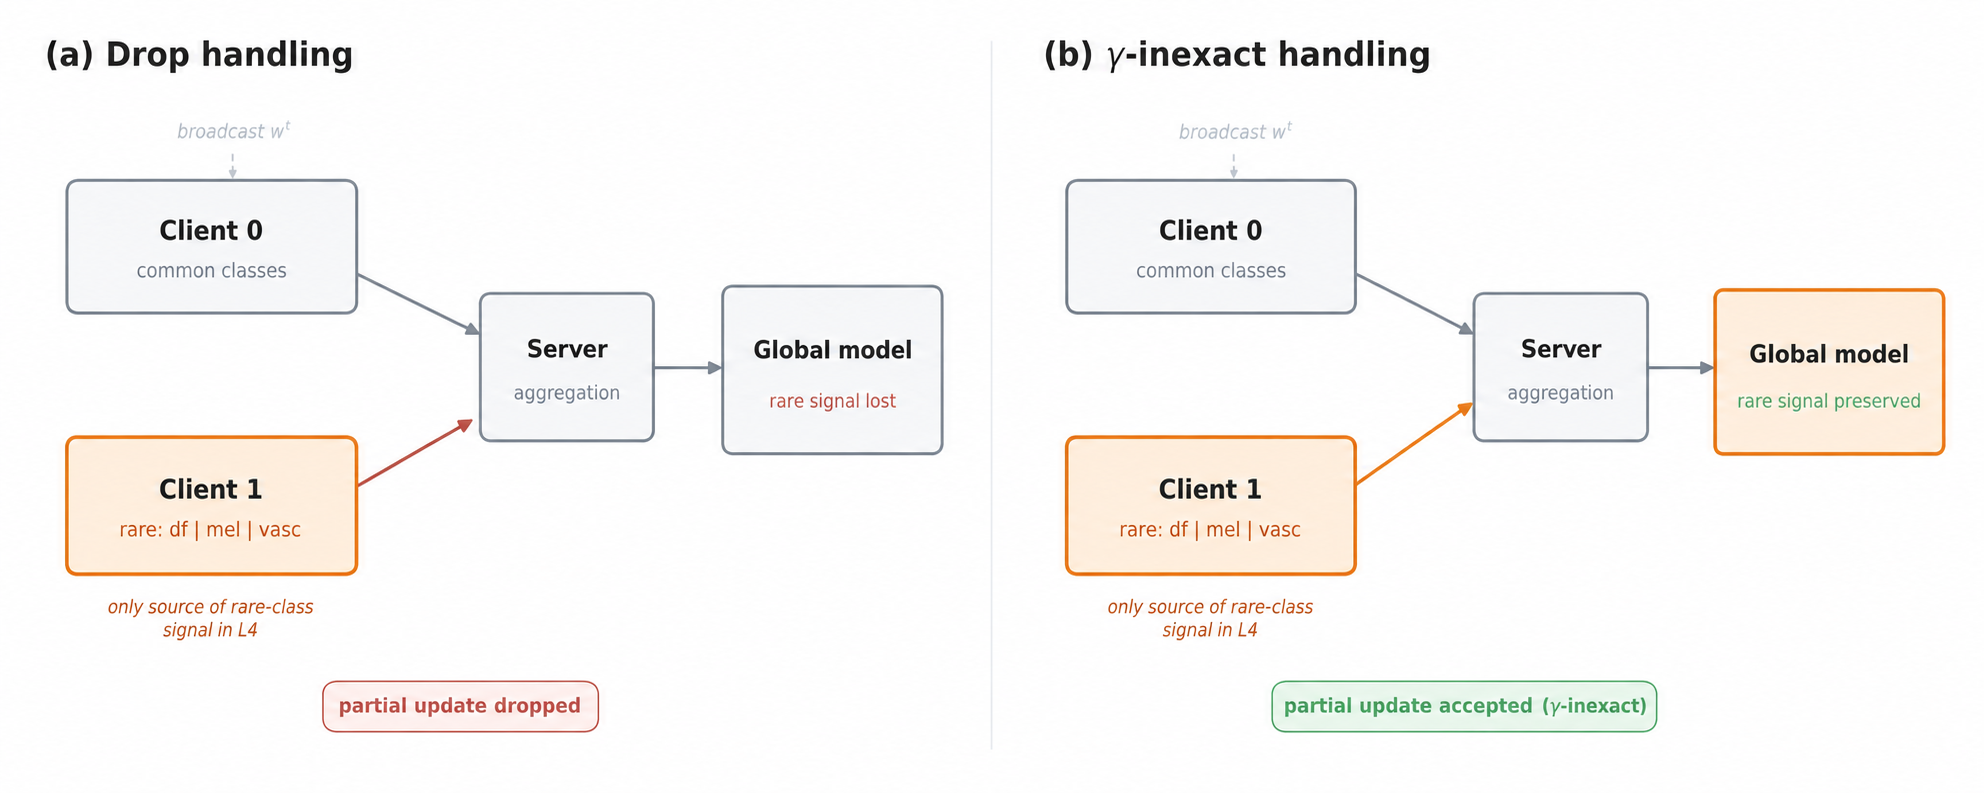
\includegraphics[width=0.90\textwidth]{F_signal_flow_gamma_inexact_improved.png}
\caption{Rare-client signal flow under drop and $\gamma$-inexact partial-update
handling in the L4 partition. Client~1 uniquely holds melanoma, dermatofibroma,
and vascular examples. Under \textbf{(a)} drop handling its partial update is
discarded, so rare-class signal is lost; under \textbf{(b)} $\gamma$-inexact
handling the partial update enters aggregation and the signal is preserved. The
schematic is conceptual; the evidence in \S\ref{sec:li-straggler} concerns the
FedProx~$+$~$\gamma$-inexact protocol in this design.}
\label{fig:signal-flow-gamma}
\end{figure}

The \emph{four-condition decomposition} runs on L4 under Regime~B with the
fixed-straggler schedule ($E_{\max} = 20$, $E_{\textrm{straggler}} = 5$ on
Client~1, the rare-class holder), $n = 3$ matched seeds per cell. Holding the
partition and schedule fixed isolates the drop-vs-accept axis from any per-round
variability, so the only quantities that change between the four cells are the optimiser
(FedAvg vs FedProx) and the partial-update protocol (drop vs $\gamma$-inexact); the
full cell-by-cell design grid is tabulated in Appendix~\ref{app:supp-tables}
(Table~\ref{tab:four-condition-design}). The design deliberately
omits a FedAvg $+$ $\gamma$-inexact cell, so attributing the rare-class-rescue effect
to the $\gamma$-inexact protocol (rather than to the proximal term alone) is a
claim about the \emph{FedProx $+$ $\gamma$-inexact} protocol, not about
$\gamma$-inexact acceptance in isolation.

Three further system-asymmetry regimes build on this. The \emph{perfect-storm}
stress keeps L4/Regime~B but raises straggling to a random fraction $0.9$,
comparing FedAvg+drop with FedProx+$\gamma$-inexact at $\mu \in \{1.0, 0.01\}$
($n = 3$); because its schedule and arms differ from the four-condition design it
is reported as a stress demonstration of the same ordering. The
\emph{learning-rate-asymmetry} envelope keeps Client~0 at
$\textrm{lr} = 0.01$ and varies Client~1 across six ratios from $1{:}1$ to $50{:}1$
($\textrm{lr}_1 \in \{0.01, 0.005, 0.002, 0.001, 0.0005, 0.0002\}$), weakening the
rare client's update magnitude \emph{without dropping it} and so separating the
``silent client'' failure mode from the ``smaller-step'' one. The
\emph{random-$\tau$ FedNova stress} runs on
the 7-client engineered partition under Regime~A with random-straggler fraction
$0.5$, $n = 10$ --- not an L4 experiment --- deliberately making $\tau_i$ a
per-round random variable --- time-varying local work that
\citet{wang2020fednova} analyse in principle, here stressed empirically
together with extreme rare-class imbalance.


\subsection{Loss-side interventions}
\label{sec:method-losses}

The loss-side comparators test a falsification hypothesis: if FedProx's advantage
is really a disguised class-imbalance correction, a direct loss-level correction
should match or exceed it on the same partition. Three losses are compared on the
L4 substrate: plain cross-entropy (the unweighted baseline); weighted CE with
inverse-frequency weights $w_c = (1/n_c)\cdot C / \sum_j (1/n_j)$ normalised so
$\sum_c w_c = C$; and focal loss \citep{lin2017focal} ($\gamma = 2$,
inverse-frequency $\alpha_c$). The focal comparator uses this repository's
class-balanced variant, in which the modulating factor is computed from the
$\alpha$-weighted cross-entropy rather than from unweighted log-probabilities, so
it is an empirical loss-side comparison. Weighted CE intervenes in per-class loss during local training while FedProx
intervenes in aggregation, so if FedProx were class re-weighting in disguise,
weighted CE would close the gap on its own. This comparator set is run only on L4.

\section{Experiment families}
\label{sec:method-roadmap}

Table~\ref{tab:experiment-families} maps the eleven experiment families to the
Results sections they support; the Results chapter follows it as a single argument
rather than a list of detached experiments. L4 is the controlled-mechanism
substrate (five rows); L1 appears once but is the load-bearing negative control for
the $\gamma$-inexact rescue mechanism (\S\ref{sec:li-straggler}).

\begin{table}[H]
\centering
\small
\caption[Experiment families and the Results sections they support]{Experiment families and the Results sections they support. The
table bridges the design choices defined in §\ref{sec:method-problem}--§\ref{sec:method-losses}
and Results (Chapter~\ref{ch:results}). Each Results section examines
one row or a group of rows; none is presented as a detached standalone
experiment.}
\label{tab:experiment-families}
\resizebox{\textwidth}{!}{%
\begin{tabular}{l p{0.18\linewidth} p{0.22\linewidth} p{0.28\linewidth} l}
\toprule
Experiment family                & Federation / partition                       & Algorithms / protocols                                  & What it tests                                                                 & Results §                                       \\
\midrule
IID control                      & 7-client IID                                 & FedAvg vs FedProx, $n = 10$                              & Falsify FedProx-helps-without-heterogeneity                                  & §\ref{sec:statistical-heterogeneity}            \\
Engineered statistical-het       & 7-client balanced-paired                     & FedAvg vs FedProx, both runtimes, $n = 10$               & Headline $\Delta$ under engineered label skew                                & §\ref{sec:statistical-heterogeneity}            \\
Robustness partitions            & 7-client Dirichlet / specialist              & FedAvg vs FedProx, $n = 10$                              & Test engineered direction outside its framing                                & §\ref{sec:statistical-heterogeneity}            \\
Node-pinned L4 control           & 2-client L4, single compute node             & FedAvg vs FedProx, $n = 3$ matched                       & Isolate cross-node CUDA non-determinism                                       & §\ref{sec:statistical-heterogeneity}            \\
$\mu$ sensitivity                & 7-client balanced-paired                     & FedProx at $\mu \in \{0, 0.001, 0.01, 0.1, 1.0\}$, $n = 10$ & Locate proximal-coefficient peak; show large-$\mu$ harm                      & §\ref{sec:mu-sensitivity}                       \\
Li-style four-condition          & 2-client L4 and L1 (control)                 & FedAvg/FedProx $\times$ drop/$\gamma$-inex, $n = 3$       & Isolate proximal-only from $\gamma$-inex contribution                         & §\ref{sec:li-straggler}                         \\
Perfect-storm                    & 2-client L4, batch $10$, momentum $0$, $90\%$ random stragglers & FedAvg+drop vs FedProx+$\gamma$-inex ($\mu \in \{1.0, 0.01\}$), $n = 3$ & Stress demonstration of the four-condition ordering                        & §\ref{sec:li-straggler}                         \\
LR asymmetry                     & 2-client L4, 6 ratios $1{:}1$ to $50{:}1$    & FedAvg, FedProx, FedNova, $n = 3$ per ratio              & FedNova robustness under deterministic LR skew                                & §\ref{sec:lr-asymmetry}                         \\
FedNova random-$\tau$            & 7-client balanced-paired, $f_{\textrm{straggle}} = 0.5$ & FedNova vs system\_het\_random FA/FP, $n = 10$           & Random-$\tau$ straggler stress under rare-class imbalance             & §\ref{sec:lr-asymmetry}                         \\
Loss-side correction             & 2-client L4                                  & FedAvg/FedProx $\times$ CE / weighted CE / focal, $n = 3$ & Test whether FedProx is a disguised class-imbalance corrector                & §\ref{sec:rare-class-collapse}                  \\
Mechanism diagnostics            & cross-protocol pool of L4 runs               & update-norm trajectories, protocol-flip audit             & Drift-control mechanism evidence; reporting-protocol robustness               & §\ref{sec:mechanism-robustness}                  \\
\bottomrule
\end{tabular}%
}
\end{table}

\noindent{\footnotesize Seed counts vary across experiments because compute
availability varied; each experiment's seed count is reported transparently in the
table above.}


%% =============================================================================
%% RESULTS
%% =============================================================================

\chapter{Results}
\label{ch:results}


%%%%%%%%%%%%%%%%%%%%%%%%%%%%%%%%%%%%%%%%%%%%%%%%%%%%%%%%%%%%%%%%%%%%%%%%%%%%%%%
%% Evaluation setting and reporting protocol
%%%%%%%%%%%%%%%%%%%%%%%%%%%%%%%%%%%%%%%%%%%%%%%%%%%%%%%%%%%%%%%%%%%%%%%%%%%%%%%

% =============================================================================
% Evaluation setting and reporting protocol
% RARE_IDX = {dermato, melanoma, vascular} (canonical).
% =============================================================================

Every configuration is evaluated by test macro-F1 at the best-validation checkpoint
(\S\ref{sec:method-metrics}): on DermaMNIST, where melanocytic nevi account for
$66.9\,\%$ of the data, accuracy saturates at the
majority floor and hides rare-class failure, whereas macro-F1 weights all seven
classes equally. Three seed tiers are used throughout: $n=10$ paired seeds for
headline comparisons, $n=3$ as directional evidence for mechanism probes, and
single-seed pilots labelled as such, with no significance test applied to the
$n=3$ directional probes; the full metric hierarchy and reporting protocol are
tabulated in Appendix~\ref{app:supp-tables} (Table~\ref{tab:reporting-protocol}).

The results proceed from weakest to strongest stress: statistical heterogeneity,
the proximal coefficient, straggler asymmetry, learning-rate asymmetry and FedNova,
rare-class collapse, and mechanism checks.


%%%%%%%%%%%%%%%%%%%%%%%%%%%%%%%%%%%%%%%%%%%%%%%%%%%%%%%%%%%%%%%%%%%%%%%%%%%%%%%
%% Statistical heterogeneity alone gives limited optimiser separation
%%%%%%%%%%%%%%%%%%%%%%%%%%%%%%%%%%%%%%%%%%%%%%%%%%%%%%%%%%%%%%%%%%%%%%%%%%%%%%%

% =============================================================================
% Statistical heterogeneity alone gives limited separation
% =============================================================================

\section{Weak separation under statistical heterogeneity}
\label{sec:statistical-heterogeneity}

This first result asks whether statistical heterogeneity alone is enough to
separate FedAvg and FedProx; the IID split serves as the negative control.
Under an IID partition (Flower, $n=10$ paired seeds), FedAvg and FedProx
differ by $\Delta = -0.007$ macro-F1 (FA $0.585$, FP $0.578$, FN $0.577$) ---
within seed noise. We treat this as a negative control: statistical
heterogeneity is a necessary condition for any FedAvg--FedProx gap on this
benchmark.

On the engineered balanced-paired seven-client partition, three estimates ($n=10$
paired seeds each; Table~\ref{tab:stat-het-headline}) agree on sign and bracket the
magnitude at $0.01$--$0.03$: the central headline is the Flower paired
$\Delta = +0.007$ (7/10 wins, full provenance), with the $\mu$-sweep peak
($+0.013$) and the pure-PyTorch reference ($+0.027$, 9/10 wins) as cross-runtime
corroboration.

The pure-PyTorch $+0.027$ is concentrated in two minority classes --- melanoma
and actinic keratoses carry $61\%$ and $36\%$ of the macro-F1 advantage --- while
the other five classes, including the invariant mel-nevi, are flat
(Figure~\ref{fig:engineered-per-class}). The gain is concentrated in the
rebalancing of two minority classes.

Three further partitions replicate the small-magnitude finding --- Dirichlet
$\alpha = 0.1$, specialist 1-of-7 ($n=10$ each), and the multi-seed node-pinned L4
control ($n=3$), all with small positive $\Delta$
(Table~\ref{tab:stat-het-headline}). The single-seed
heterogeneity-ladder pilot at L4 gives $\Delta = -0.030$, but that deficit is one
rare-class (vascular) outcome on one seed and the $n=3$ node-pinned promotion
averages it out. (Dirichlet aggregates use regenerated raw-JSON summaries.)

On the engineered partition, FedProx reduces test-macro-F1 SD from $0.025$
to $0.014$ ($-45\,\%$), reaches validation macro-F1 $= 0.40$ in $9.8$ vs
$12.7$ rounds ($1.3\times$ speed-up), and shows a paired mid-training peak
$\Delta = +0.094$ at round 50 that closes to $+0.007$ by round 150. These
trajectory characteristics are documented for the engineered partition only.

Statistical heterogeneity alone produces small, runtime-sensitive separation
(Table~\ref{tab:stat-het-headline}). The
next question is whether the proximal coefficient $\mu$ itself explains when
FedProx helps.


% =============================================================================
% statistical heterogeneity and runtime sensitivity
% =============================================================================

\begin{table}[H]
\centering
\caption{Statistical heterogeneity and runtime sensitivity: test macro-F1
(mean $\pm$ sample SD where shown) for FedAvg vs FedProx across six settings ---
IID, the engineered partition through both runtimes plus the $\mu$-peak,
Dirichlet $\alpha=0.1$, specialist 1-of-7, and the node-pinned L4 control.
IID, Dirichlet, and specialist values are from regenerated raw-JSON aggregates.}
\label{tab:stat-het-headline}
\resizebox{\textwidth}{!}{%
\begin{tabular}{lccccccl}
\toprule
Setting              & Runtime       & Clients & $n$ & FedAvg              & FedProx             & $\Delta$ & Note \\
\midrule
IID                  & Flower        & 7       & 10  & $0.585 \pm 0.020$   & $0.578 \pm 0.020$   & $-0.007$ & negative control \\
Engineered (pure)    & pure-PyTorch  & 7       & 10  & $0.481 \pm 0.025$   & $0.508 \pm 0.014$   & $+0.027$ & 9/10 wins; partial provenance \\
Engineered (Flower)  & Flower        & 7       & 10  & $0.496$             & $0.503$             & $+0.007$ & 7/10 wins; \textbf{central} \\
Dirichlet $\alpha=0.1$ & Flower      & 7       & 10  & $0.480 \pm 0.036$   & $0.488 \pm 0.034$   & $+0.008$ & regenerated raw-JSON \\
Specialist 1-of-7    & Flower        & 7       & 10  & $0.437 \pm 0.024$   & $0.445 \pm 0.017$   & $+0.008$ & --- \\
Node-pinned L4       & Flower        & 2       & 3   & $0.492 \pm 0.019$   & $0.497 \pm 0.022$   & $+0.005$ & multi-seed L4 control \\
\bottomrule
\end{tabular}%
}
\end{table}




% =============================================================================
% engineered partition per-class trajectories
% =============================================================================

\begin{figure}[H]
\centering
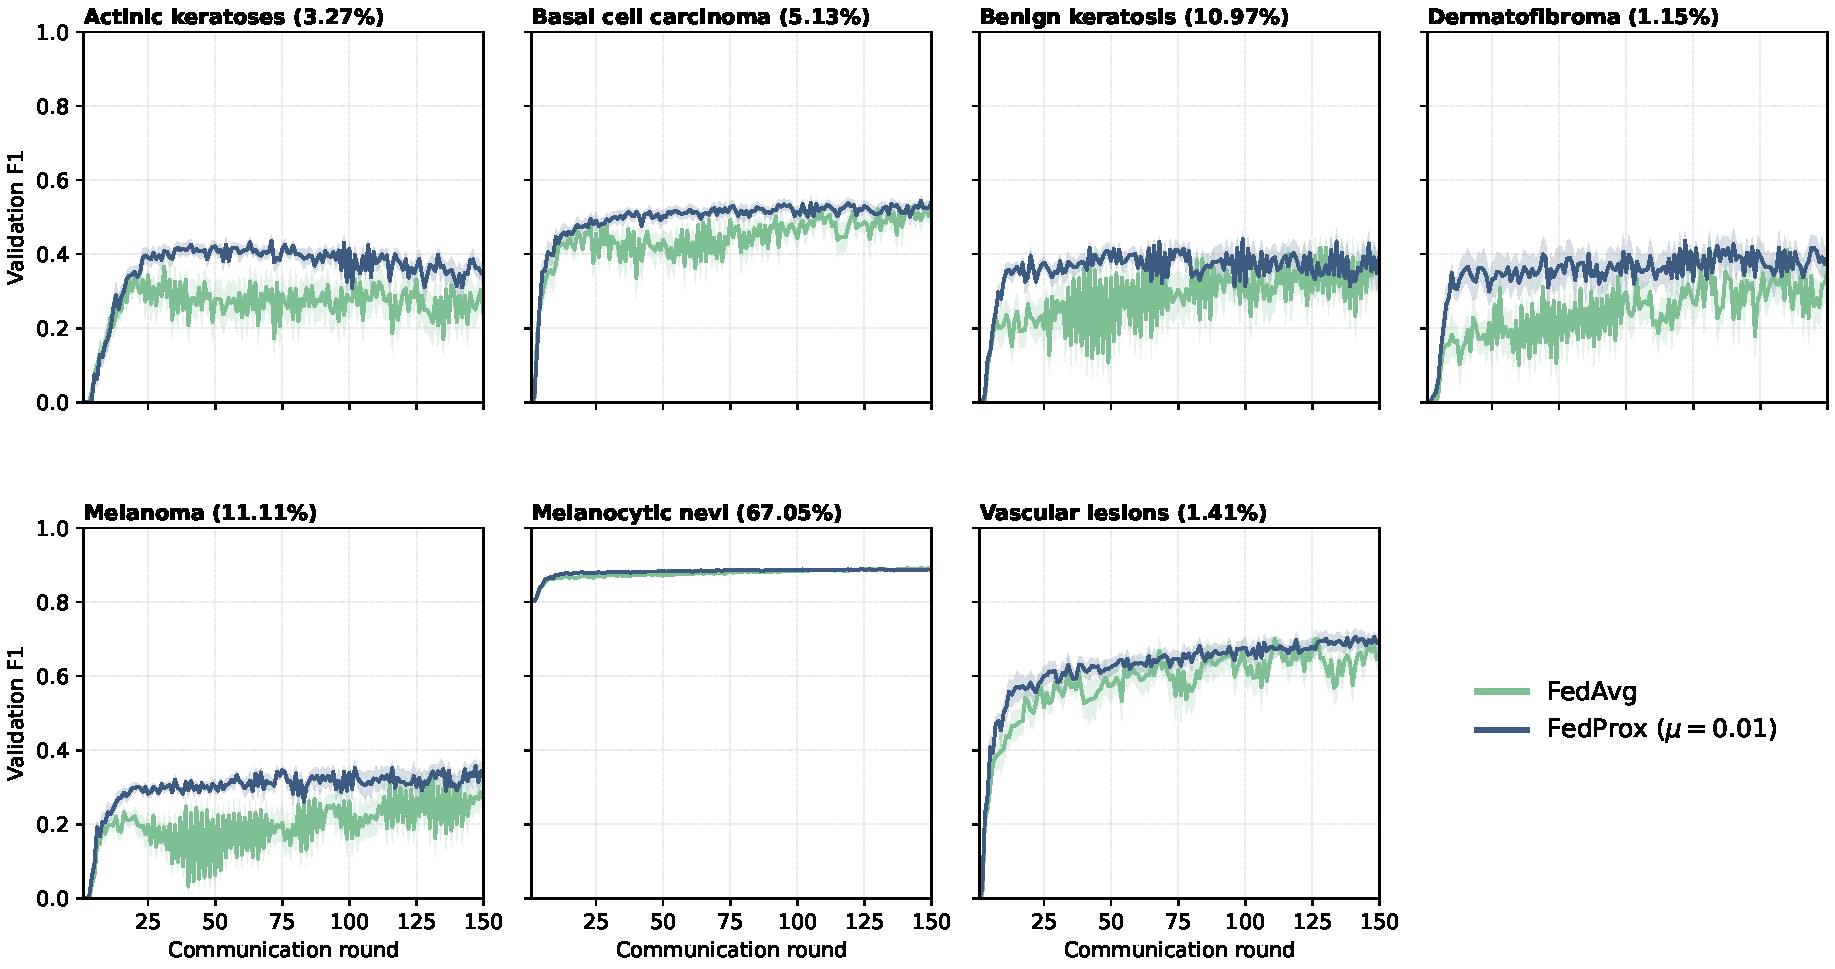
\includegraphics[width=\textwidth]{F_engineered_per_class.pdf}
\caption{Per-class validation F1 trajectories on the engineered partition from
the \emph{pure-PyTorch} headline runs, $n = 10$ paired seeds (FedAvg vs FedProx,
mean $\pm 1$ SEM bands). By
mid-training the melanoma and actinic-keratoses panels show non-overlapping
FedAvg/FedProx bands --- the two minority classes that carry the engineered
FedProx advantage --- while the other five classes overlap throughout 150
rounds, including the dominant mel-nevi panel, which stays invariant near its
prevalence saturation.}
\label{fig:engineered-per-class}
\end{figure}


%%%%%%%%%%%%%%%%%%%%%%%%%%%%%%%%%%%%%%%%%%%%%%%%%%%%%%%%%%%%%%%%%%%%%%%%%%%%%%%
%% mu sensitivity: the proximal term helps only in a narrow range
%%%%%%%%%%%%%%%%%%%%%%%%%%%%%%%%%%%%%%%%%%%%%%%%%%%%%%%%%%%%%%%%%%%%%%%%%%%%%%%

% =============================================================================
% mu sensitivity
% =============================================================================

\section{Proximal coefficient: a narrow useful range}
\label{sec:mu-sensitivity}

The next question is whether the proximal coefficient $\mu$ --- the one knob
distinguishing FedProx from FedAvg --- governs the advantage, and whether larger
$\mu$ helps under heterogeneity. A five-cell sweep ($\mu \in \{0.001, 0.01, 0.1,
1.0\}$ against the $\mu = 0$ FedAvg baseline; engineered partition, $n=10$ paired
seeds) traces a clear inverted-$U$ (Table~\ref{tab:mu-sweep},
Figure~\ref{fig:mu-inverted-u}): peak near $\mu = 0.01$, below baseline by
$\mu = 0.1$, catastrophic at $\mu = 1.0$.

The peak is at $\mu = 0.01$ ($\Delta = +0.013$, 6/10 wins), essentially tied with
$\mu = 0.001$; by $\mu = 0.1$ FedProx falls below baseline, and at $\mu = 1.0$ it
collapses ($\Delta = -0.074$, 0/10 wins; Table~\ref{tab:mu-sweep}). The $0.09$
macro-F1 spread between best and worst $\mu$ is an order of magnitude larger than
any partition-level $\Delta$ in \S\,\ref{sec:statistical-heterogeneity}.

The $\mu$-sweep peak $\Delta = +0.013$ exceeds the
\S\,\ref{sec:statistical-heterogeneity} Flower paired $\Delta = +0.007$
because the sweep selects best-of-five on the same seeds; the two estimates
bracket the same small effect at $+0.005$ to $+0.015$.

The practical region of useful $\mu$ on this benchmark is a single decade
around $0.01$. The expectation that larger $\mu$ should be preferred under
stronger statistical heterogeneity is not supported here --- a benchmark
observation specific to this setting.

The $\mu = 1.0$ deficit concentrates in the rare and minority classes while the
dominant mel-nevi is essentially invariant (Table~\ref{tab:mu-per-class}) --- the
same rare-class shape as the dropped-straggler and asymmetric-LR failures
(\S\,\ref{sec:rare-class-collapse}), via a different mechanism
(over-regularisation rather than under-aggregation). Because $\mu$ alone is
sensitive and harmful when large, the much larger FedProx gains under straggler
protocols (\S\,\ref{sec:li-straggler}) cannot be attributed to the proximal
coefficient itself.


% =============================================================================
% mu-sensitivity sweep
% =============================================================================

\begin{table}[H]
\centering
\caption{$\mu$ sensitivity on the engineered partition, $n=10$ paired
seeds per cell. ``Wins'' is paired comparisons where FedProx exceeds
FedAvg on the matched seed.}
\label{tab:mu-sweep}
\begin{tabular}{cccc}
\toprule
$\mu$    & macro-F1 (mean $\pm$ SD)   & $\Delta$ vs FedAvg & Wins / 10 \\
\midrule
$0$      & $0.493 \pm 0.020$          & ---               & ---  \\
$0.001$  & $0.504 \pm 0.021$          & $+0.011$          & 6    \\
$0.01$   & $\mathbf{0.506 \pm 0.017}$ & $\mathbf{+0.013}$ & 6    \\
$0.1$    & $0.479 \pm 0.017$          & $-0.014$          & 2    \\
$1.0$    & $0.419 \pm 0.013$          & $-0.074$          & 0    \\
\bottomrule
\end{tabular}
\end{table}


% =============================================================================
% mu-sensitivity curve
% =============================================================================

\begin{figure}[H]
\centering
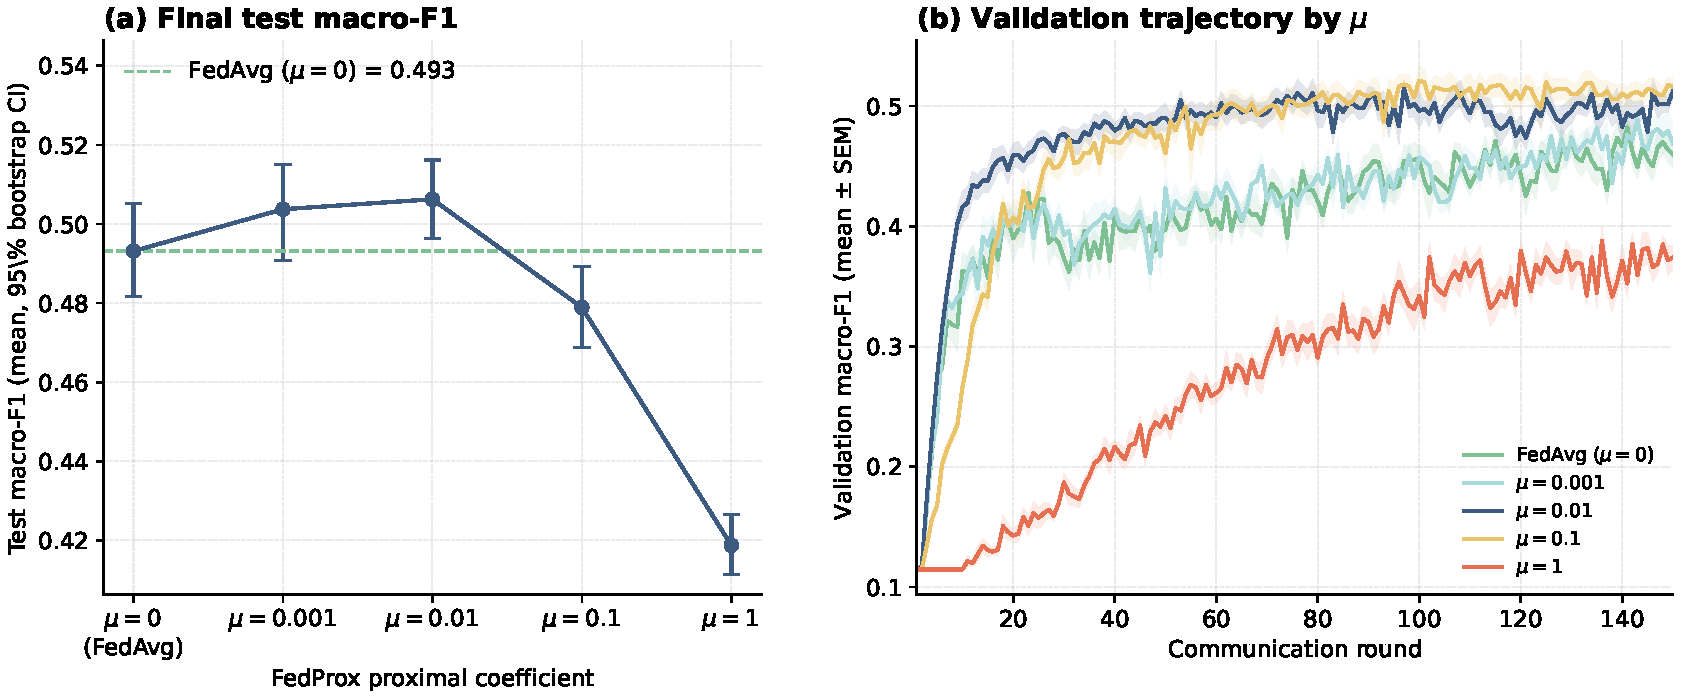
\includegraphics[width=0.85\textwidth]{F_mu_sensitivity_outcome_and_convergence.pdf}
\caption{Inverted-$U$ $\mu$ sensitivity curve on the engineered partition
($n=10$ per cell). $x$-axis: $\mu$ on $\log_{10}$ scale across
$\{0.001, 0.01, 0.1, 1.0\}$, FedAvg baseline as dashed reference line at
$0.493$. $y$-axis: test macro-F1 with $\pm 1$ SD whiskers.}
\label{fig:mu-inverted-u}
\end{figure}


%%%%%%%%%%%%%%%%%%%%%%%%%%%%%%%%%%%%%%%%%%%%%%%%%%%%%%%%%%%%%%%%%%%%%%%%%%%%%%%
%% Li-style straggler asymmetry (CENTREPIECE)
%%%%%%%%%%%%%%%%%%%%%%%%%%%%%%%%%%%%%%%%%%%%%%%%%%%%%%%%%%%%%%%%%%%%%%%%%%%%%%%

% =============================================================================
% Centrepiece
% =============================================================================

\section{Straggler asymmetry: \texorpdfstring{$\gamma$}{gamma}-inexact handling, not the proximal term}
\label{sec:li-straggler}

This section presents the central result of the thesis. Every preceding
section has shown the FedAvg--FedProx gap to be small; here it becomes
large, and a controlled four-condition decomposition attributes that gap
to its true cause --- not the proximal regulariser FedProx is named for,
but the $\gamma$-inexact partial-update handling it is conventionally
paired with. This is what turns the thesis from an optimiser comparison
into a regime map.

Before decomposing the mechanism, we first checked whether stragglers alone
create a FedProx advantage. They do not: in a 7-client IID random-straggler
control FedProx is slightly worse than FedAvg ($\Delta = -0.013$ macro-F1,
$n = 10$), but replacing the IID split with a heterogeneous one under the same
straggler protocol reverses the sign ($\Delta = +0.017$, $n = 10$). The advantage
appears only when slow or partially updated clients also carry non-redundant
class information; the next experiment isolates that mechanism in a two-client L4
decomposition with the rare-class client as the fixed straggler.

We next isolate the mechanism in a two-client L4 four-condition experiment,
with $n=3$ matched seeds (Table~\ref{tab:li-decomp-l4}). In this setting,
Client 1 contains the rare-class signal and is made the fixed straggler. The
four cells separate two effects that are otherwise bundled together in
FedProx-style straggler experiments: the proximal term and the decision to
accept or drop a straggler's partial update.

\begin{table}[H]
\centering
\caption{Li-style four-condition decomposition at L4 (two-client; $n=3$
matched seeds; mean $\pm$ sample SD across seeds).}
\label{tab:li-decomp-l4}
\small
\begin{tabular}{lcc}
\toprule
Condition                                       & Test macro-F1                & Rare-class F1 \\
\midrule
FedAvg, no straggler                            & $0.485 \pm 0.028$            & $0.316 \pm 0.060$ \\
FedAvg + drop                                   & $0.364 \pm 0.009$            & $0.000 \pm 0.000$ \\
FedProx + drop (control)                        & $0.368 \pm 0.005$            & $0.000 \pm 0.000$ \\
FedProx + $\gamma$-inexact                      & $\mathbf{0.479 \pm 0.010}$   & $\mathbf{0.291 \pm 0.018}$ \\
\bottomrule
\end{tabular}

\smallskip
\noindent\textit{Decomposition:} proximal-only $= 0.368 - 0.364 = +0.004$;
$\gamma$-inexact $= 0.479 - 0.368 = +0.111$; total $= +0.115$. Rare-F1 is
the mean over $\mathrm{RARE\_IDX} = \{\text{dermato}, \text{melanoma},
\text{vascular}\}$: both drop-handling cells sit at zero and only
FedProx+$\gamma$-inexact recovers it.
\end{table}

Dropping the straggler removes class information rather than merely slowing
training: FedAvg falls from $0.485$ to $0.364$. Adding the proximal term while
still dropping changes almost nothing ($+0.004$), whereas accepting the partial
update recovers nearly the full baseline ($+0.111$). About $96\%$ of the $+0.115$
gain is therefore $\gamma$-inexact acceptance, not the proximal term. Because the
design omits a FedAvg+$\gamma$-inexact cell, this is evidence for the
FedProx+$\gamma$-inexact protocol specifically; the standalone effect of
$\gamma$-inexact acceptance is left for future isolation.

Figure~\ref{fig:val-curves-extreme-gaps}~(A) shows the same result over
training: the FedAvg+drop and FedProx+drop trajectories overlap for all 150
rounds, while FedProx+$\gamma$-inexact separates from both around round 30 and
stabilises near $0.48$.

\begin{figure}[H]
\centering
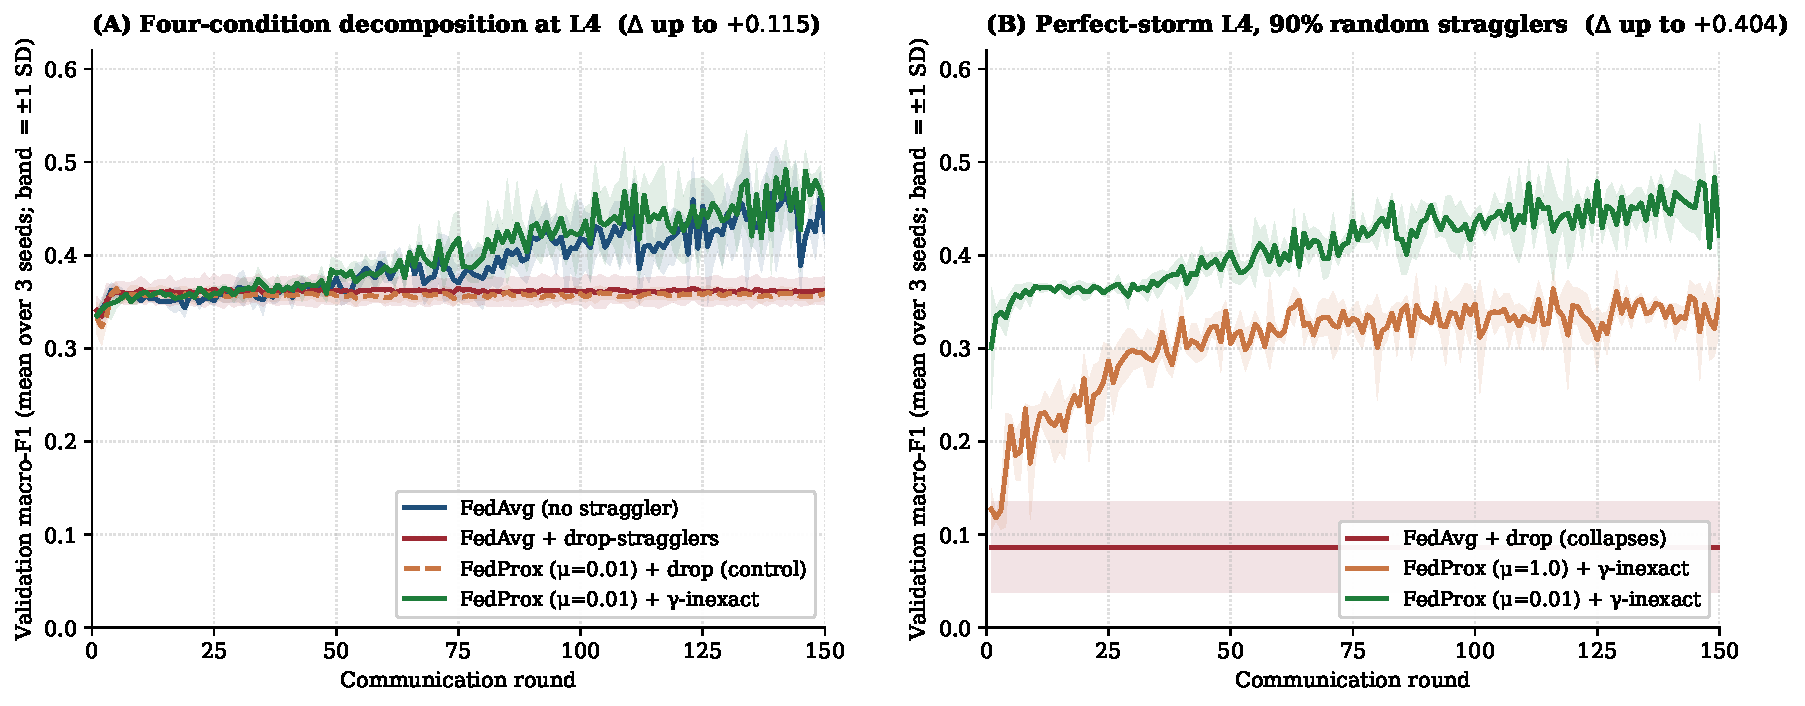
\includegraphics[width=\textwidth]{F_val_curves_extreme_gaps.pdf}
\caption[Validation-macro-F1 trajectories: four-condition and perfect-storm]{Validation macro-F1 trajectories at the two settings with the
largest FedAvg vs FedProx differences (mean over three seeds; shaded
bands are $\pm 1$ sample SD). (A) The four-condition
decomposition at L4: the FedAvg+drop and FedProx+drop trajectories overlap
throughout the 150 rounds; only FedProx+$\gamma$-inexact separates and
recovers towards the no-straggler baseline ($\Delta$ up to $+0.115$).
(B) Perfect-storm L4 with $90\%$ random stragglers: FedAvg+drop flatlines
at its round-1 validation value, so the selected checkpoint is effectively
the untrained model, while FedProx+$\gamma$-inexact climbs to
$0.491$ at $\mu = 0.01$ ($\Delta$ up to $+0.404$ --- the largest
FedProx--FedAvg gap measured in the thesis).}
\label{fig:val-curves-extreme-gaps}
\end{figure}

Per-class trajectories (Figure~\ref{fig:l4-per-class-grid}) localise the gain to
the rare classes: mel-nevi stays near $0.89$ under all four conditions, while
dermatofibroma, melanoma, and vascular collapse under both drop cells and recover
only under FedProx+$\gamma$-inexact --- the mechanism is rare-class learning, not
a broad improvement.

\begin{figure}[H]
\centering
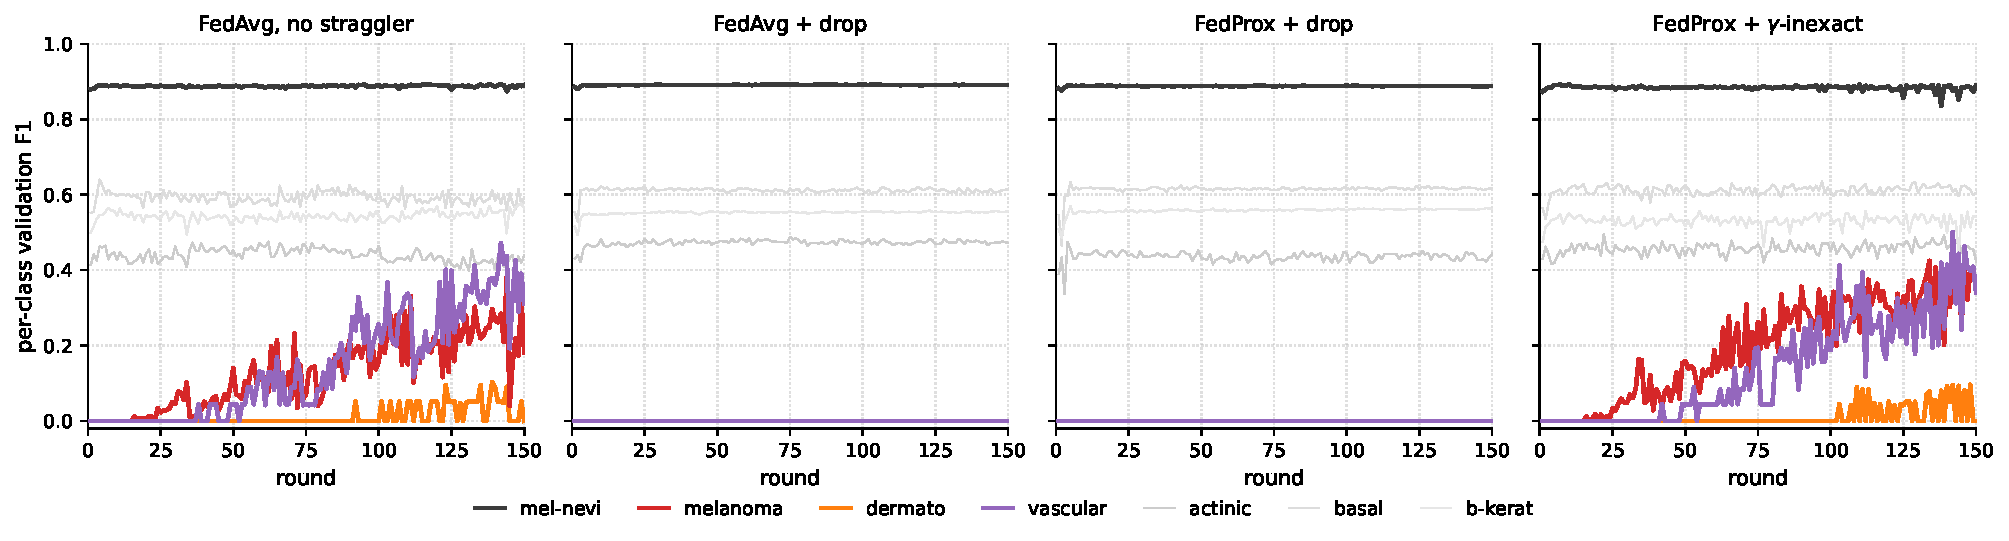
\includegraphics[width=\textwidth]{F_l4_four_condition_per_class_grid.pdf}
\caption[Per-class F1 under the four-condition L4 decomposition]{Per-class validation F1 trajectories under the four conditions of
the L4 decomposition (Table~\ref{tab:li-decomp-l4}); mean over three seeds.
The majority class (mel-nevi) stays near $0.89$ in every cell, so the
aggregate improvement is not driven by the dominant class. The three rare
classes (dermatofibroma, melanoma, vascular) flatline at zero under \emph{both}
drop-handling cells --- FedAvg+drop and FedProx+drop alike, so the proximal term
alone does not rescue them --- and recover only under FedProx+$\gamma$-inexact,
identifying $\gamma$-inexact acceptance, not the proximal term, as the locus of
the mechanism.}
\label{fig:l4-per-class-grid}
\end{figure}

The perfect-storm experiment stresses the same ordering rather than re-deriving
it: on the same L4 setting with a $90\%$ per-round random-straggler rate (batch
$10$, no momentum), FedAvg+drop flatlines at its round-1 value --- best-val
selects the untrained init, mean test macro-F1 $0.087 \pm 0.049$ --- while
FedProx+$\gamma$-inexact recovers to $0.365 \pm 0.023$ at $\mu = 1.0$ and
$0.491 \pm 0.003$ at $\mu = 0.01$, the latter the largest FedProx--FedAvg gap in
the thesis ($\Delta = +0.404$; Figure~\ref{fig:val-curves-extreme-gaps}B). The
mechanism is the one the L4 decomposition isolated (Figure~\ref{fig:signal-flow-gamma}),
pushed to its limit; the smaller $\mu$ wins because looser anchoring leaves more
rare-class learning signal per round. This is a magnitude demonstration, not a
second causal decomposition: the schedule and arms differ from the four-condition
design, and FedAvg+drop collapses too completely for a clean
$\gamma$-inexact-vs-proximal split.

Finally, the L1 control tests whether partial-update acceptance is simply a better
generic straggler policy. It is not. L1 uses the same four-condition design but with
identical label proportions, so the split changes quantity, not class information.
All four cells are then nearly flat (Table~\ref{tab:li-decomp-l1}): accepting the
partial update adds only $+0.012$, against $+0.111$ at L4.

\begin{table}[H]
\centering
\caption{L1 cross-partition control: same four-condition design as
Table~\ref{tab:li-decomp-l4} but on the L1 partition (quantity-only
heterogeneity, JS divergence $\approx 0$); $n=3$ matched seeds, test
macro-F1 mean $\pm$ sample SD with rare-class F1.}
\label{tab:li-decomp-l1}
\small
\begin{tabular}{lcc}
\toprule
Condition                                       & Test macro-F1        & Rare-class F1 \\
\midrule
FedAvg, no straggler                            & $0.601 \pm 0.010$    & $0.530 \pm 0.008$ \\
FedAvg + drop                                   & $0.599 \pm 0.006$    & $0.539 \pm 0.012$ \\
FedProx + drop (control)                        & $0.593 \pm 0.022$    & $0.537 \pm 0.039$ \\
FedProx + $\gamma$-inexact                      & $0.605 \pm 0.009$    & $0.556 \pm 0.014$ \\
\bottomrule
\end{tabular}

\smallskip
\noindent\textit{Decomposition (vs L4 in parentheses):}
proximal-only $= 0.593 - 0.599 = -0.006$ (L4: $+0.004$);
$\gamma$-inexact $= 0.605 - 0.593 = +0.012$ (L4: $+0.111$);
drop-cost $= 0.601 - 0.599 = +0.002$ (L4: $+0.121$). At L1 every rare-F1
cell sits in $0.53$--$0.56$, whereas at L4 the two drop cells fall to zero
and only $\gamma$-inexact recovers rare-F1 (to $0.29$).
\end{table}

The L4/L1 contrast is therefore the key mechanism evidence. At L4, the
dropped client carries class information the other client does not have, so
accepting its partial update rescues rare-class learning. At L1, the dropped
client carries no unique class signal, so there is little to rescue. The
straggler mechanism is not generic drift control; it matters when system
heterogeneity suppresses statistically unique rare-class information.

The straggler experiments isolate one axis of system asymmetry.
Section~\ref{sec:lr-asymmetry} asks whether persistent learning-rate
imbalance --- a different axis --- changes the optimiser ranking.


%%%%%%%%%%%%%%%%%%%%%%%%%%%%%%%%%%%%%%%%%%%%%%%%%%%%%%%%%%%%%%%%%%%%%%%%%%%%%%%
%% Learning-rate asymmetry reveals FedNova regime-dependence
%%%%%%%%%%%%%%%%%%%%%%%%%%%%%%%%%%%%%%%%%%%%%%%%%%%%%%%%%%%%%%%%%%%%%%%%%%%%%%%

% =============================================================================
% Learning-rate asymmetry, FedNova regime-dependence
% =============================================================================

\section{Learning-rate asymmetry and FedNova regime-dependence}
\label{sec:lr-asymmetry}

This experiment tests a different form of system heterogeneity from
\S\,\ref{sec:li-straggler}. There, the rare-class client was slow and its
partial update could be dropped. Here, the rare-class client is not dropped:
it still participates in every round, but its learning rate is made smaller.
The question is whether an optimiser can preserve rare-class learning when
the rare client's update becomes progressively weaker.

The experiment is run on L4. Client 0 is the dominant client and keeps
$\textrm{lr}=0.01$ throughout. Client 1 holds the rare classes and is assigned
one of six smaller learning rates, producing asymmetry ratios from 1:1 to
50:1. Each ratio is tested with FedAvg, FedProx, and FedNova using $n=3$
matched seeds per cell, giving $54$ runs in total. Test macro-F1 across the
six-ratio envelope is reported in Table~\ref{tab:lr-envelope}.

\begin{table}[H]
\centering
\caption[Learning-rate-asymmetry envelope at L4]{Learning-rate-asymmetry envelope at L4, $n=3$ matched seeds per cell.
Client~0 (dominant) holds $\textrm{lr} = 0.01$ throughout; Client~1
(rare-class holder) takes the smaller rate that sets each ratio. Columns are
test macro-F1 for the three optimisers and the FedNova advantage over FedAvg
and FedProx. FedNova (bold) leads at every ratio and stays flat across the
envelope, while FedAvg and FedProx plateau at the rare-class floor by 5:1.}
\label{tab:lr-envelope}
\resizebox{0.9\textwidth}{!}{%
\begin{tabular}{cccccccc}
\toprule
Ratio & Client 0 lr & Client 1 lr & FedAvg & FedProx & FedNova & FN$-$FA & FN$-$FP \\
\midrule
 1:1  & $0.0100$ & $0.0100$ & $0.457$ & $0.491$ & $\mathbf{0.509}$ & $+0.052$ & $+0.018$ \\
 2:1  & $0.0100$ & $0.0050$ & $0.425$ & $0.462$ & $\mathbf{0.526}$ & $+0.101$ & $+0.064$ \\
 5:1  & $0.0100$ & $0.0020$ & $0.375$ & $0.392$ & $\mathbf{0.504}$ & $+0.129$ & $+0.112$ \\
10:1  & $0.0100$ & $0.0010$ & $0.369$ & $0.369$ & $\mathbf{0.501}$ & $+0.132$ & $+0.132$ \\
20:1  & $0.0100$ & $0.0005$ & $0.367$ & $0.372$ & $\mathbf{0.486}$ & $+0.119$ & $+0.114$ \\
50:1  & $0.0100$ & $0.0002$ & $0.367$ & $0.367$ & $\mathbf{0.498}$ & $\mathbf{+0.131}$ & $\mathbf{+0.131}$ \\
\bottomrule
\end{tabular}%
}
\end{table}

The pattern is clear (Table~\ref{tab:lr-envelope}). FedAvg and FedProx both
degrade as soon as Client~1's learning rate is reduced and plateau near $0.367$
macro-F1 by 5:1 --- the rare-class floor, where the model still learns the
dominant-client distribution but rare-class learning has largely collapsed.
FedNova behaves differently, holding $0.486$--$0.526$ across the full 1:1--50:1
envelope; even at 50:1 it reaches $0.498$ against $0.367$ for both FedAvg and
FedProx, a $+0.131$ macro-F1 gap. Rare-class F1 confirms this is not a macro-F1
artefact: it is near zero for FedAvg and FedProx by 10:1 (FA $0.016$, FP $0.010$)
but stays around $0.35$ for FedNova across the envelope
(Figure~\ref{fig:lr-asymmetry-envelope}).

\begin{figure}[H]
\centering

\includegraphics[width=\textwidth]{F_asymmetric_lr_L4.pdf}
\caption{Learning-rate asymmetry envelope at L4, $n=3$ per cell. Two
panels: test macro-F1 and rare-class F1 (mean over dermato, melanoma,
vascular) vs the Client 1 LR ratio on a $\log_{10}$ axis from 1:1 to 50:1.
FedAvg and FedProx plateau at the rare-class floor; FedNova stays flat
across the envelope. Exact macro-F1 values and FedNova deltas are in
Table~\ref{tab:lr-envelope}.}
\label{fig:lr-asymmetry-envelope}
\end{figure}

The 5:1 cell is where the metric choice earns its keep. Raw accuracy would prefer
FedAvg ($0.753$) over FedNova ($0.726$), yet FedAvg's macro-F1 ($0.375$, rare-F1
$\approx 0.02$) shows it has lost the rare classes while FedNova has not ($0.504$,
rare-F1 $\approx 0.37$): the accuracy gap is small only because both still classify
mel-nevi ($66.9\,\%$ of the test set) correctly. This is why
\S\,\ref{sec:method-metrics} ranks by macro-F1, not accuracy.

The interpretation is that a reduced learning rate makes Client~1's local model
move less, so its update carries weaker rare-class information. FedAvg does not
correct this, and the FedProx proximal term cannot restore an update that is
already too small; FedNova, by normalising updates by effective local work,
preserves Client~1's contribution in this deterministic-asymmetry setting.

The update-norm logs are mechanism-consistent: at 5:1 Client~1's update retains
$0.91$ of its 1:1 size under FedNova but only about half ($0.47$ FedAvg, $0.50$
FedProx), so the rare-client contribution is preserved under normalisation and
attenuated without it (\S\,\ref{sec:mechanism-robustness}).

FedNova's success here is not universal: it fails under random-$\tau$ straggler
heterogeneity, where the amount of local work varies randomly from round to
round. On the same 7-client engineered partition as the
\S\,\ref{sec:li-straggler} screening comparison (Regime~A, per-round random
schedule; \emph{not} an L4 experiment), FedNova obtains only
$0.237 \pm 0.094$ macro-F1, far below the matching FedAvg and FedProx cells
($n = 10$: FA $0.493 \pm 0.028$, FP $0.510 \pm 0.017$). Best-val selection masks
the severity: three of ten seeds already sit at the majority-class-only baseline
($\approx 0.114$, predicting mel-nevi for every image) at best-val. The final
validation histories show all ten runs ending below $0.20$ macro-F1, with nine of
ten reaching the strict mel-nevi-only pattern; because final \emph{test} metrics
were not saved for this sweep, this is reported as a validation-trajectory failure
mode rather than a final-test estimate.

This contrast is the section's main point: FedNova is empirically robust under
deterministic learning-rate asymmetry but brittle under random, noisy local work.
The mechanism is work-normalisation: FedNova normalises by effective
local work ($\tau$), and this normalised aggregation interacts favourably with a
stable, persistently weakened update but amplifies unstable partial updates under
random $\tau$; the precise cause is left
to future work, so FedNova is best read as regime-dependent rather than universally
superior (Table~\ref{tab:fednova-regime}).

\begin{table}[H]
\centering
\small
\caption{FedNova across the two system-heterogeneity regimes: persistent
deterministic learning-rate asymmetry ($n=3$) versus random per-round $\tau$
stragglers ($n=10$). Test macro-F1; the mechanism reading is given in the
text.}
\label{tab:fednova-regime}
\begin{tabular}{p{0.22\linewidth}p{0.32\linewidth}p{0.38\linewidth}}
\toprule
FedNova regime & Result & Interpretation \\
\midrule
Persistent LR asymmetry & macro-F1 holds $0.49$--$0.53$ across 1:1--50:1 & Empirically robust; robustness from work-normalised ($\tau$) aggregation \\
Random-$\tau$ stragglers & macro-F1 $= 0.237 \pm 0.094$; 3/10 majority-only at best-val, 9/10 by the final validation round (no final test saved) & $\tau$-normalisation amplifies noisy partial updates (empirical; cause left to future work) \\
\bottomrule
\end{tabular}
\end{table}

Across these regimes, optimiser gaps become large only under specific stress, and
the failing protocols fail in a clinically specific way --- they lose rare-class
sensitivity. The next section shows this failure usually appears as rare-class
images routed into the dominant mel-nevi class.


%%%%%%%%%%%%%%%%%%%%%%%%%%%%%%%%%%%%%%%%%%%%%%%%%%%%%%%%%%%%%%%%%%%%%%%%%%%%%%%
%% Rare-class collapse into mel-nevi
%%%%%%%%%%%%%%%%%%%%%%%%%%%%%%%%%%%%%%%%%%%%%%%%%%%%%%%%%%%%%%%%%%%%%%%%%%%%%%%

% =============================================================================
% Rare-class collapse + loss-side correction
% =============================================================================

\section{Rare-class collapse and the loss-side comparison}
\label{sec:rare-class-collapse}

The previous sections show \emph{when} the optimiser gap becomes large; this
section asks what those failures look like at the class level, and whether the
FedProx advantage is merely class-imbalance correction in disguise.

\paragraph{Per-class collapse.}

The low-macro-F1 cells in \S\S\,\ref{sec:li-straggler}--\ref{sec:lr-asymmetry}
fail the same way --- on the rare classes, not the majority. Synthesising
per-class optimiser differences across the whole study, the large
FedProx$-$FedAvg (and FedNova$-$FedAvg) per-class F1 gaps sit almost entirely in
the rare-class columns and almost entirely in the system-heterogeneity cells
(Figure~\ref{fig:cross-experiment-per-class}). The failure itself is misrouting:
rare-class images are predicted as mel-nevi. Mean rare-to-mel-nevi
misrouting (over dermato, melanoma, vascular) ranges from $24\,\%$ in the
best protocol (perfect-storm FP $\mu = 0.01$, $n=3$) to $67\,\%$ in the
worst (perfect-storm FA+drop, $n=3$), and $28\,\%$ even under the IID
Flower negative control ($n=10$) --- a class-imbalance saturation that the
FL protocol preserves or amplifies but does not itself create. A confusion-matrix
view of this rare-to-mel-nevi routing across the four-condition cells is given in
Appendix~\ref{app:diagnostics} (Figure~\ref{fig:l4-confusion-appendix}).

The D1 5:1 cell isolates the optimiser dimension: melanoma \emph{recall} is
$1.20\,\%$ (FedAvg), $6.13\,\%$ (FedProx), and $46.34\,\%$ (FedNova) --- the same
disease across three regimes spanning two orders of magnitude. Because macro-F1
weights all seven classes equally, losing one class moves it by $\approx 0.057$,
the order of the entire engineered $\Delta$ (\S\,\ref{sec:statistical-heterogeneity}).
The same shape recurs across aggregation dropout, learning-rate asymmetry, and the
$\mu = 1.0$ over-regularisation cell (\S\,\ref{sec:mu-sensitivity}).

\begin{table}[H]
\centering
\small
\caption{Rare-class collapse across four representative cells spanning the
straggler and learning-rate-asymmetry axes ($n=3$ each). Columns: Rare-F1
(mean F1 over dermato, melanoma, vascular), melanoma recall, melanoma F1, and
rare-to-mel-nevi misrouting. Mel.\ recall reports whether melanoma is recovered
at all; mel.\ F1 adds the precision penalty.}
\label{tab:collapse-cells}
\resizebox{\textwidth}{!}{%
\begin{tabular}{p{0.15\linewidth} p{0.12\linewidth} c c c c p{0.29\linewidth}}
\toprule
Protocol                  & Algorithm & Rare-F1 & Mel.\ recall & Mel.\ F1 & Misrouting & Interpretation \\
\midrule
Perfect-storm + drop      & FedAvg    & $0.000$ & $0.00\,\%$  & $0.00\,\%$  & $67\,\%$   & Rare client dropped; flatline \\
Perfect-storm + $\gamma$  & FedProx ($\mu=0.01$) & $0.327$ & $38.27\,\%$ & $34.46\,\%$ & $24\,\%$ & $\gamma$-inex preserves rare signal \\
D1 5:1 LR asymmetry       & FedAvg    & $0.036$ & $1.20\,\%$  & $2.28\,\%$  & $51\,\%$   & Rare client under-weighted; gradual erosion \\
D1 5:1 LR asymmetry       & FedNova   & $0.359$ & $46.34\,\%$ & $36.74\,\%$ & $26\,\%$   & Robust to the stable weakened update \\
\bottomrule
\end{tabular}%
}
\end{table}

\noindent
These four cells (Table~\ref{tab:collapse-cells}) span instant-collapse and
gradual-erosion modes across straggler and LR-asymmetry axes; the misrouting
rate co-varies with rare-F1 across all four.


\paragraph{Collapse modes.}

The collapse takes two temporal forms of one mechanism: an \emph{instant}
collapse when updates are dropped wholesale (perfect-storm FedAvg+drop flatlines
at its round-1 value, mean $0.087 \pm 0.049$), and a \emph{gradual} erosion when
they are merely under-weighted (D1 5:1 drifts $0.457 \to 0.375$ with rare-F1
falling in lockstep).


\paragraph{Loss-side imbalance correction (weighted CE and focal loss).}

To test whether the FedProx advantage might be class-imbalance correction
in disguise, we ran FedAvg and FedProx at L4 with three loss functions
($n=3$ per cell): plain cross-entropy, class-weighted CE with
inverse-frequency weights, and focal loss ($\gamma = 2$). The results are
in Table~\ref{tab:loss-side}.

\begin{table}[H]
\centering
\caption{Loss-side imbalance correction at L4 ($n=3$ per cell). Cells are
test macro-F1 $\pm$ sample SD with rare-class F1 in parentheses; the strongest
cell is bold.}
\label{tab:loss-side}
\begin{tabular}{lccc}
\toprule
Algorithm & CE & Weighted CE & Focal \\
\midrule
FedAvg  & $0.477 \pm 0.002$ ($0.285$) & $\mathbf{0.505 \pm 0.023}$ ($\mathbf{0.367}$) & $0.467 \pm 0.002$ ($0.317$) \\
FedProx & $0.478 \pm 0.016$ ($0.291$) & $0.503 \pm 0.014$ ($0.346$)                   & $0.476 \pm 0.022$ ($0.304$) \\
\bottomrule
\end{tabular}
\end{table}

Three points follow (Table~\ref{tab:loss-side}). Weighted CE is the strongest
loss-side correction: FedAvg+wCE ($0.505$) marginally exceeds FedProx+CE
($0.478$), the CE-to-wCE step alone raising FedAvg rare-F1 by $+0.082$. Focal
raises rare-F1 but lowers macro at $\gamma=2$. And FedProx adds little on top of
either loss --- FP+wCE sits inside FA+wCE's seed SD --- so FedProx acts as a
drift/protocol intervention complementary to direct loss-side correction.
This does not conflict with \S\,\ref{sec:li-straggler}: $\gamma$-inexact acceptance
restores aggregation under straggler-induced signal loss while weighted CE
re-weights rare classes during local training, so they act at different pipeline
stages and are combinable in principle, though tested only separately here
($n=3$, L4).

The rare-class collapse documented here is clinically \emph{motivated},
not clinically \emph{validated}: DermaMNIST is a $28 \times 28$-pixel
benchmark, and external validation on real multi-site workflows remains future
work. The next section turns to the
per-round update-norm activity behind these per-class outcomes.


% =============================================================================
% cross-experiment per-class FedProx-vs-FedAvg F1 differences
% =============================================================================

\begin{figure}[H]
\centering

\includegraphics[width=\textwidth]{F_cross_experiment_per_class.pdf}
\caption[Cross-experiment per-class FedProx/FedNova vs FedAvg differences]{Cross-experiment synthesis: per-class FedProx$-$FedAvg (or
FedNova$-$FedAvg) test-F1 differences across the principal experiment cells ---
statistical-heterogeneity baselines, the heterogeneity ladder, the four-condition
L4 decomposition, perfect-storm, asymmetric LR, and node-pinned L4. The mel-nevi
column is near zero everywhere (both optimisers already classify the majority
correctly) and the statistical-heterogeneity rows are near zero throughout; large
positive differences appear in the rare-class columns (dermatofibroma, melanoma,
vascular) precisely in the system-heterogeneity cells.}
\label{fig:cross-experiment-per-class}
\end{figure}


%%%%%%%%%%%%%%%%%%%%%%%%%%%%%%%%%%%%%%%%%%%%%%%%%%%%%%%%%%%%%%%%%%%%%%%%%%%%%%%
%% Mechanism and robustness checks
%%%%%%%%%%%%%%%%%%%%%%%%%%%%%%%%%%%%%%%%%%%%%%%%%%%%%%%%%%%%%%%%%%%%%%%%%%%%%%%

% =============================================================================
% Mechanism and robustness checks
% =============================================================================

\section{Mechanism and robustness}
\label{sec:mechanism-robustness}

After the main regime contrasts, these diagnostics check whether the
drift-control reading is consistent with update-level behaviour and whether the
optimiser ranking is robust to reporting choices.

\paragraph{Update-norm activity.}

Update norms ($\lVert \Delta w \rVert$, the size of the client update returned to
the server) are used here only as a supporting diagnostic, not as causal proof.
Two facts emerge. First, FedProx does what its proximal term intends: on the
engineered partition the mean per-round update norm falls from $1.523$
(FedAvg) to $1.029$ (FedProx, $\mu=0.01$), a $32\%$ reduction
(Figure~\ref{fig:update-norms}; update-norm diagnostic logs were available for
$9$ FedAvg, $8$ FedProx and $7$ FedNova seeds, not the full ten). This is a local-training effect and does not
contradict \S\,\ref{sec:li-straggler}, where the straggler-regime gain came from
accepting the rare client's partial update rather than from the proximal term.

Second, as a separate cross-protocol correlation (not shown in
Figure~\ref{fig:update-norms}), update size tracks rare-class performance only
within a controlled protocol. Pooled across 78 L4 runs, larger dominant-client
update norms correlate with higher rare-class F1 (Spearman $r=+0.634$), but the
Client~1-to-Client~0 ratio does not ($r=-0.045$) because the pool mixes mechanisms.
Inside the asymmetric-LR experiment alone, rare-class F1 closely follows the rare
client's relative update strength ($r=+0.80$ FedAvg, $r=+0.87$ FedProx). These are
mechanism-consistent correlations; the main claims rest on the
controlled contrasts in \S\,\ref{sec:li-straggler} and \S\,\ref{sec:lr-asymmetry}.

\paragraph{Protocol-flip audit.}

The protocol-flip audit checks whether the algorithm ranking depends on the
reporting checkpoint (best-validation vs final round vs last-$K$ mean); a flip is
a sign change of the paired difference across these choices. Large effects do not
flip and small ones do: $0/9$ flips in the large-effect settings (Li-style
decomposition, perfect-storm) versus $3/9$ in the small-effect settings. The
centrepiece \S\,\ref{sec:li-straggler} effect ($+0.115$) and the
\S\,\ref{sec:lr-asymmetry} FedNova gap ($+0.131$) therefore survive
checkpoint choice, while the small \S\,\ref{sec:statistical-heterogeneity}
separations should be read as fragile. Several further diagnostics (the
$B$-dissimilarity proxy, training-instability metric, asymmetric-$\mu$ probe,
early-warning detector, and small-hospital case study) were examined but are not
load-bearing. Both checks support the same message: large regime-dependent effects
are robust, small symmetric-protocol differences are not.

% =============================================================================
% update-norm mechanism
% =============================================================================

\begin{figure}[H]
\centering

\includegraphics[width=0.85\textwidth]{F_update_norms.pdf}
\caption{Update-norm mechanism diagnostic. Mean per-round client update-norm
($\lVert \Delta w \rVert_2$) trajectories for FedAvg and FedProx on the
engineered non-IID partition (panel~A) and the IID mechanism-null partition
(panel~B), with light $\pm1$ SEM bands across seeds. Update-norm logs were
available for $9$ FedAvg and $8$ FedProx seeds on the engineered partition
($10$ each on the IID partition). FedProx tracks lower update norms under the
engineered partition, consistent with the proximal term's drift-control role;
on the IID partition the two trajectories sit low and close together, as
expected when the mechanism is largely inactive. This is a supporting
diagnostic.}
\label{fig:update-norms}
\end{figure}


%%%%%%%%%%%%%%%%%%%%%%%%%%%%%%%%%%%%%%%%%%%%%%%%%%%%%%%%%%%%%%%%%%%%%%%%%%%%%%%
%% Integrated summary of findings
%%%%%%%%%%%%%%%%%%%%%%%%%%%%%%%%%%%%%%%%%%%%%%%%%%%%%%%%%%%%%%%%%%%%%%%%%%%%%%%

% =============================================================================
% Integrated summary of findings
% verbatim per guide sec 1.
% =============================================================================

%% (tab:final-claims) were relocated into the Discussion (\S4.1). The duplicated
%% signal-flow restatement was dropped per the restructuring plan.


%%%%%%%%%%%%%%%%%%%%%%%%%%%%%%%%%%%%%%%%%%%%%%%%%%%%%%%%%%%%%%%%%%%%%%%%%%%%%%%
%% Limitations
%%%%%%%%%%%%%%%%%%%%%%%%%%%%%%%%%%%%%%%%%%%%%%%%%%%%%%%%%%%%%%%%%%%%%%%%%%%%%%%

% =============================================================================
% Limitations
% =============================================================================

%% Conclusion chapter (\S4.2 Limitations).


%% =============================================================================
%% END OF RESULTS BODY
%% =============================================================================


%% =============================================================================
%% CHAPTER 6: DISCUSSION AND CONCLUSION
%% =============================================================================
\chapter{Discussion and Conclusion}
\label{ch:discussion}

\section{Discussion}
\label{sec:disc}

The results are best read not as a contest between three optimisers but as a map
of when each preserves rare-class signal in the global model. Optimiser
performance is regime-dependent for one reason: rare-class performance depends on
whether the rare client's contribution survives aggregation, and different
optimisers protect or forfeit it under different heterogeneity. This single rule
organises the six experiments across the regimes studied.


Read through that rule, the findings cohere. Statistical heterogeneity alone
separates FedAvg and FedProx only slightly and runtime-sensitively
(\S\ref{sec:statistical-heterogeneity}), too fragile to justify a universal
preference, and the proximal coefficient is sharply tuned: useful near
$\mu = 0.01$ but harmful at $\mu = 1.0$, where it damages exactly the rare classes
(\S\ref{sec:mu-sensitivity}). This already indicates that the proximal term acts
on local drift, not on whether a client's signal is admitted.

The L4/L1 decomposition makes the point precise (\S\ref{sec:li-straggler}): under straggler
asymmetry the FedProx advantage of about $+0.115$ macro-F1 comes almost entirely
($+0.111$) from $\gamma$-inexact acceptance of the straggler's partial update and
only $+0.004$ from the proximal term, while the matched L1 control --- where the
suppressed client carries nothing unique --- collapses the effect, confirming that
admitting the partial update matters only when that client is the sole source of
rare-class signal.

FedNova fits the same picture from another angle
(\S\ref{sec:lr-asymmetry}): it is empirically robust under deterministic
learning-rate asymmetry (an advantage of about $+0.131$ macro-F1 at the most
extreme ratio) but amplifies noise and collapses to roughly $0.237$ under random,
round-to-round straggling --- a robustness best read as its work-normalised
($\tau$) aggregation interacting favourably with a \emph{stable} weakened update,
not as direct learning-rate normalisation.

Finally, class-weighted cross-entropy matches or exceeds FedProx with plain cross-entropy on the symmetric
partition (\S\ref{sec:rare-class-collapse}), locating imbalance correction as a
loss-side layer distinct from the aggregation-and-protocol layer where FedProx
acts; the two address different failure modes and could in principle be combined.
This loss-stage comparison does not explain away the separate $\gamma$-inexact
straggler result, which acts at the protocol/aggregation stage.

These findings refine rather than contradict prior work. FedAvg
\citep{mcmahan2017fedavg} behaves as expected when clients are well matched; for
FedProx \citep{li2020fedprox}, the decomposition indicates --- within this
benchmark and this simulated protocol --- that the straggler-regime benefit is
carried mainly by inexact-update acceptance rather than by the proximal term, an
attribution to the FedProx-plus-$\gamma$-inexact protocol as configured here
rather than a claim that the method underperforms; and for FedNova
\citep{wang2020fednova} --- whose analysis explicitly covers time-varying
local work --- the random-$\tau$ collapse is an empirical brittleness in this
small, rare-class-imbalanced regime, not a flaw in that analysis. No result
here should be read as refuting these analyses. The clinical reading stays
cautious: rare lesions collapsing into melanocytic nevi is the shared failure
mode, but DermaMNIST is a $28 \times 28$ benchmark, so this is clinically
motivated, not validated.

The headline findings and supporting diagnostics, with explicit strength labels,
are collected in Table~\ref{tab:final-claims}.

\begin{table}[H]
\centering
\small
\caption[Final claim--evidence summary]{Final claim--evidence summary. Strength labels: \emph{strong}
= multi-seed, mechanism-isolable, checkpoint-robust; \emph{medium} =
multi-seed but small effect or single-protocol; \emph{exploratory} =
correlational, single-protocol, or $n=3$ without mechanism isolation.}
\label{tab:final-claims}
\begin{tabular}{p{3.0cm}p{5.0cm}p{1.7cm}p{3.6cm}}
\toprule
Claim & Evidence & Strength & Implication \\
\midrule
FedProx not free under IID & Flower IID $\Delta = -0.007$ ($n=10$) & strong & Reach for FedProx only when heterogeneity exists \\
Stat-het alone gives fragile separation & Flower engineered $\Delta = +0.007$ (7/10 wins, $n=10$) & medium & Do not recommend FedProx on partition alone \\
$\mu$ must be tuned & Sweep $n=10$: peak $+0.013$ at $\mu = 0.01$; $-0.074$ at $\mu = 1.0$ & strong & Default $\mu = 0.01$; do not raise under heterogeneity \\
$\gamma$-inexact dominates straggler gain & L4 four-condition $n=3$: total $+0.115$, $\gamma$-inex $+0.111$; L1 control $+0.012$ & medium--strong & Use FedProx + $\gamma$-inexact under straggler protocols \\
FedNova regime-dependent & LR envelope: FN holds $0.49$--$0.53$ across 1:1--50:1 ($n=3$); random-$\tau$ collapses to $0.237$ ($n=10$; 9/10 majority-only by the final validation round) & medium--strong & Prefer FedNova under persistent LR asymmetry, not under random-$\tau$ \\
Rare-class collapse is the clinically relevant benchmark failure mode & Misrouting $24\,\%$--$67\,\%$; D1 5:1 melanoma recall $= 1.2$/$6.1$/$46.3\,\%$ (F1 $2.3$/$10.8$/$36.7\,\%$, $n=3$) & strong & Report per-class metrics; macro-F1 alone hides it \\
wCE competes with FedProx & L4 $n=3$: FA+wCE $0.505$ vs FP+CE $0.478$ & medium & Loss-side rebalancing is a competitive intervention \\
Update-norms support drift-control reading & Engineered: FA $1.523$ vs FP $1.029$ ($-32\,\%$); cross-protocol $r = +0.634$ & exploratory & Update norms corroborate the drift-control reading \\
\bottomrule
\end{tabular}
\end{table}

\section{Limitations}
\label{sec:limitations}

Several scope conditions bound these conclusions. First, the study is a controlled
benchmark simulation rather than a clinical deployment. All experiments use
DermaMNIST at $28 \times 28$ resolution, stragglers are simulated through
local-epoch budgets rather than wall-clock deadlines, and the L1/L4 partitions are
stylised stress regimes designed to isolate mechanism behaviour. These choices make
the failure modes easier to attribute, but they also mean that the results should
be read as a regime map for controlled heterogeneity settings, not as a validated
claim about real hospital networks or full-resolution dermatology workflows.

Second, the evidence is strongest where the experiments are replicated and more
exploratory where compute limited the number of seeds. The headline comparisons use
larger seed counts, while the mechanism probes use three matched seeds and are
reported as directional rather than significance-tested. The heterogeneity ladder is
a single-seed exploratory pilot. In addition, the engineered partition shows the
same direction of FedProx--FedAvg separation across the pure-PyTorch and Flower
runtimes, but with different magnitudes, so the robust conclusion is directional
rather than an exact effect-size claim.

Third, the optimiser and evaluation space is deliberately limited. The comparison
covers FedAvg, FedProx, and FedNova, but not variance-reduced or adaptive federated
methods such as SCAFFOLD \citep{karimireddy2020scaffold}, FedAdam, or FedYogi
\citep{reddi2021adaptive}. Evaluation is based on argmax predictions, macro-F1, and
per-class diagnostics; AUC, calibration, and cross-client fairness measures are not
reported.

These limitations mainly restrict the breadth of the claims rather than the internal
comparison. The thesis does not establish a universal optimiser ranking or a
clinically validated recommendation. It instead identifies where rare-class signal
is preserved or lost under controlled forms of statistical and system heterogeneity.
Directions for addressing these constraints are set out in the Conclusion.

\section{Conclusion}
\label{sec:conc}

This thesis asked not whether a federated optimiser is best for imbalanced medical
image classification but \emph{when} each preserves rare-class performance. The
answer is a regime map governed by a single rule: rare-class performance is
preserved when rare-client signal reaches the global model. Statistical
heterogeneity alone yields only a fragile FedProx--FedAvg separation (RQ1); under
straggler asymmetry the FedProx advantage is carried mainly by $\gamma$-inexact
partial-update handling rather than the proximal term, and only when the
suppressed client holds unique rare-class signal (RQ2); FedNova is
regime-dependent, robust under deterministic learning-rate asymmetry but brittle
under random stragglers (RQ3); and rare-class collapse into melanocytic nevi is
the common failure mode, with weighted cross-entropy a competitive loss-side
alternative for rare-class preservation rather than evidence that the
$\gamma$-inexact straggler effect is class-imbalance correction in disguise (RQ4). Concretely, in the
perfect-storm stress this margin is large: FedProx with $\gamma$-inexact
acceptance reaches $0.491$ test macro-F1 where FedAvg with straggler dropping
collapses to $0.087$ --- the thesis's largest FedAvg--FedProx gap, $\Delta =
+0.404$. Future work should combine
$\gamma$-inexact aggregation with a weighted-cross-entropy local objective, which
were tested only separately here; validate the map on higher-resolution and
additional datasets with real wall-clock straggler protocols; add variance-reduced
and adaptive optimisers; and log per-client validation to quantify fairness across
sites. In imbalanced medical federated learning, optimiser choice should be driven by the
heterogeneity regime: the best method is the one whose protocol keeps rare-client
signal reaching the global model.


%% =============================================================================
%% BIBLIOGRAPHY
%% =============================================================================
\bibliographystyle{plainnat}
\bibliography{references}


%% =============================================================================
%% APPENDICES
%% =============================================================================
\appendix

\chapter{Provenance, reproducibility, and supplementary diagnostics}
\label{app:repro}

\section{Code, data, and environment}
\label{app:repro-setup}

\paragraph{Code availability.}
All code accompanies this submission as the \texttt{fl\_dermamnist} repository,
released under the MIT licence (\texttt{LICENSE}); its top-level
\texttt{README.md} maps each Results section to the code, raw results, and figure
that support it, together with the commands below.

\paragraph{Data availability.}
Experiments use DermaMNIST from MedMNIST~v2 \citep{yang2023medmnistv2}, derived
from HAM10000 \citep{tschandl2018ham10000}. The data is not versioned with the
code: it is stored locally as a $64\times64$ array (\texttt{dermamnist\_64.npz})
and the loader resizes to the $28\times28$ resolution used throughout. It is
freely re-obtainable through the pinned \texttt{medmnist} package; HAM10000 is
released under CC~BY-NC~4.0.

\paragraph{Environment.}
Dependencies are pinned in \texttt{requirements.txt} (tested on Python~3.14) and
install with \texttt{pip install -r requirements.txt} from the repository root
(or \texttt{pip install -e .}\ for the \texttt{fl\_dermamnist} package in editable
mode).

\paragraph{Reproduction.}
The report's tables and figures rebuild from the saved per-run artefacts without
re-training. \texttt{bash infra/local/commands.sh sanity} runs the core
implementation guards (the FedProx $\mu=0\equiv$ FedAvg equivalence, the proximal
term, and provenance fields; the FedNova normaliser, straggler, partition, and
seeding guards run in the full \texttt{pytest} suite), and
\texttt{bash infra/local/commands.sh analyse} regenerates the thesis tables and
figures. Full hyperparameter sweeps were run on HPC via the
\texttt{infra/slurm/submit\_*.sh} launchers and are costly to re-run; the saved
outputs are the intended reproduction path.

\paragraph{Provenance.}
Every reported number traces to a raw artefact through the result-traceability
matrix (claim $\rightarrow$ section $\rightarrow$ raw files $\rightarrow$ generating
script $\rightarrow$ HPC job) and a numerical verification ledger, both under
\texttt{docs/provenance/}.

\section{Runtimes and implementation provenance}
\label{app:provenance}

The implementation modules (aggregation, the pure-PyTorch and Flower training
loops under \texttt{core/} and \texttt{runtimes/}, the partitioner, and the
FedNova/straggler strategies) and the unit-test guards are documented in the
repository README. The guards cover the proximal term, the
$\mu = 0 \Leftrightarrow$ FedAvg equivalence, the FedNova normaliser, straggler
dropping, partition determinism, and provenance fields.

Flower production runs save per-round validation histories, selected-round metrics
with a provenance dictionary (git commit, hostname, framework and Python/PyTorch
versions, timestamps), argmax prediction NPZs (used for confusion matrices and
misrouting in §\ref{sec:rare-class-collapse}), and optional update-norm logs.
Older pure-PyTorch headline runs retain histories and metrics but lack git-commit
provenance, prediction NPZs, and update-norm logs, which is why the chapter treats
them as direction-only corroboration. Every numerical claim in
Chapter~\ref{ch:results} traces to raw artefacts or freshly regenerated summaries,
never to stale committed CSVs.

\section{Supplementary tables}
\label{app:supp-tables}

These tables are referenced from the main text but relocated here to keep the
body focused on headline evidence; no values differ from the main-text claims.

\begin{table}[H]
\centering
\small
\caption{Reporting protocol and metric hierarchy. Applied uniformly across the
Results sections.}
\label{tab:reporting-protocol}
\begin{tabular}{p{0.20\linewidth} p{0.32\linewidth} p{0.40\linewidth}}
\toprule
Component               & Choice                                       & Reason \\
\midrule
Primary metric          & Test macro-F1 at best-val checkpoint         & Class-imbalanced; accuracy saturates at majority floor \\
Secondary metrics       & Per-class F1, per-class recall (confusion-matrix diagonal), rare-F1, rare-to-mel-nevi misrouting & Surface per-class failure that macro can mask; misrouting names the specific collapse mode \\
Rare-class definition   & $\{\text{dermato}, \text{melanoma}, \text{vascular}\}$ & Low support + high clinical priority (melanoma is mid-support but high-stakes) \\
$n = 10$ protocol       & Paired sign count + Wilcoxon where applicable & Headline statistical-heterogeneity comparisons \\
$n = 3$ protocol        & Directional only; no significance test       & Mechanism probes; power insufficient for $p$-values \\
$n = 1$ protocol        & Labelled ``pilot'' (single seed)             & Heterogeneity ladder; single-class seed events possible \\
Runtimes                & Flower (central), pure-PyTorch (corroboration) & Flower carries full git+update-norm provenance \\
\bottomrule
\end{tabular}
\end{table}

\begin{table}[H]
\centering
\small
\caption{Four-condition decomposition design (L4, two-client, Regime~B,
$E_{\textrm{straggler}} = 5$ on Client~1, $n = 3$ matched seeds per
cell). Holding the partition and schedule fixed across all four cells
isolates the optimiser-vs-protocol contribution. The design omits the
FedAvg + $\gamma$-inexact cell, so the $\gamma$-inexact attribution is
to the FedProx + $\gamma$-inexact \emph{protocol} rather than to
$\gamma$-inexact acceptance as a standalone universal mechanism.}
\label{tab:four-condition-design}
\resizebox{\textwidth}{!}{%
\begin{tabular}{l c c c p{0.28\linewidth}}
\toprule
Condition                            & Straggler schedule           & Partial-update handling & Proximal term & Mechanism isolated                                          \\
\midrule
FedAvg, no straggler                 & uniform ($E = 20$ everywhere) & not applicable          & --            & No-system-heterogeneity baseline                            \\
FedAvg + drop                        & fixed, Client 1 $E = 5$       & drop                    & --            & Cost of dropping the rare-class client's partial update     \\
FedProx + drop                       & fixed, Client 1 $E = 5$       & drop                    & $\mu = 0.01$  & Proximal-only contribution under matched drop handling      \\
FedProx + $\gamma$-inexact           & fixed, Client 1 $E = 5$       & accept ($\gamma$-inex)  & $\mu = 0.01$  & Additional effect of accepting the partial update           \\
\bottomrule
\end{tabular}%
}
\end{table}

\begin{table}[H]
\centering
\small
\caption{Per-class test F1 mean (at the best-validation checkpoint) across
the $\mu$ sweep on the engineered partition, $n = 10$ paired seeds per cell. SDs across seeds
range $0.003$ (mel-nevi) to $0.113$ (rare classes). ``$\Delta$ at $\mu=1.0$''
is the absolute per-class F1 deficit at the catastrophic cell relative to
the FedAvg baseline ($\mu = 0$). The deficit concentrates in rare and
minority classes; the dominant mel-nevi class is essentially invariant.
Source: \texttt{mu\_sensitivity\_flower/}.}
\label{tab:mu-per-class}
\resizebox{\textwidth}{!}{%
\begin{tabular}{lcccccc}
\toprule
Class       & $\mu = 0$ & $\mu = 0.001$ & $\mu = 0.01$ & $\mu = 0.1$ & $\mu = 1.0$ & $\Delta$ at $\mu = 1.0$ \\
\midrule
actinic     & $0.475$   & $0.470$       & $0.489$      & $0.434$     & $0.351$     & $-0.124$ \\
basal       & $0.497$   & $0.513$       & $0.497$      & $0.405$     & $0.438$     & $-0.060$ \\
b-kerat     & $0.405$   & $0.400$       & $0.423$      & $0.416$     & $0.328$     & $-0.077$ \\
dermato     & $0.259$   & $0.287$       & $0.283$      & $0.279$     & $0.158$     & $\mathbf{-0.101}$ \\
melanoma    & $0.244$   & $0.258$       & $0.304$      & $0.287$     & $0.216$     & $-0.028$ \\
mel-nevi    & $0.884$   & $0.885$       & $0.886$      & $0.886$     & $0.867$     & $-0.017$ \\
vascular    & $0.687$   & $0.713$       & $0.661$      & $0.646$     & $0.574$     & $\mathbf{-0.113}$ \\
\bottomrule
\end{tabular}%
}
\end{table}

\section{Supplementary diagnostics}
\label{app:diagnostics}

\begin{figure}[H]
\centering
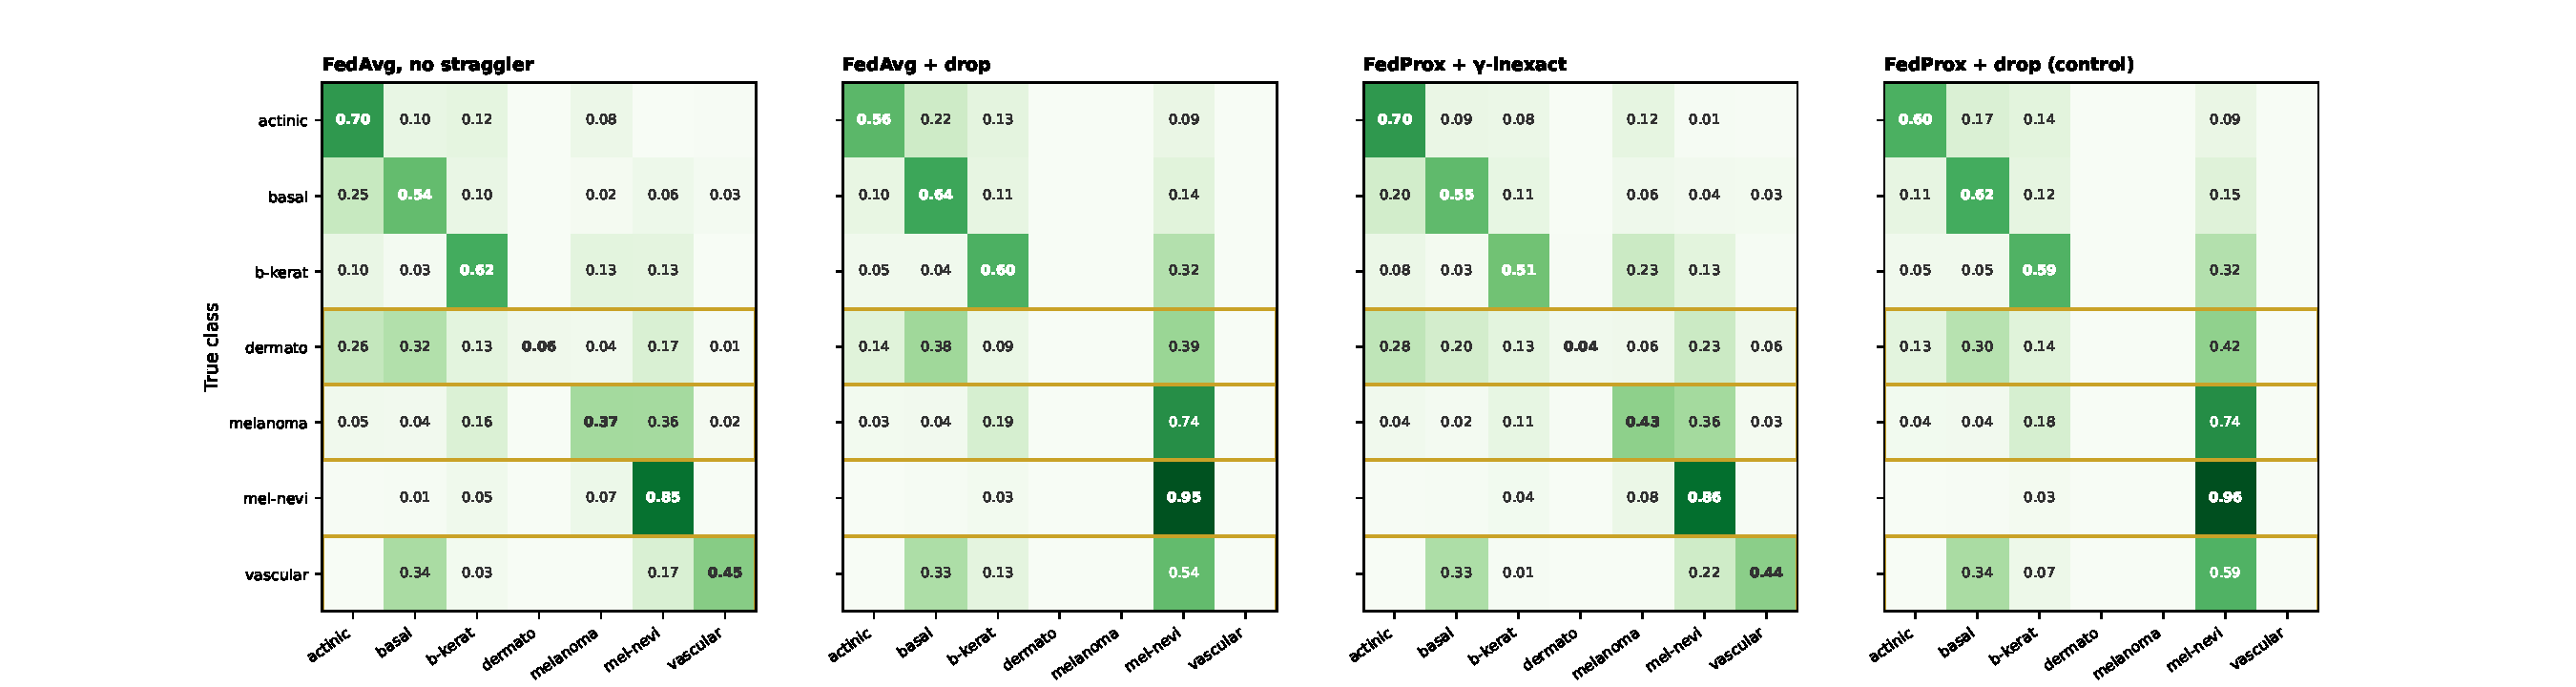
\includegraphics[width=\textwidth]{F_l4_confusion_four_condition.pdf}
\caption{Confusion-matrix diagnostic for the four-condition L4 decomposition
(row-normalised, mean over three seeds; rare classes outlined). Under drop
handling (FedAvg${}+{}$drop and FedProx${}+{}$drop), rare-class examples ---
melanoma especially --- are frequently routed into the majority mel-nevi class,
the misrouting behind the rare-class macro-F1 collapse discussed in
\S\ref{sec:rare-class-collapse}. FedProx${}+{}$$\gamma$-inexact acceptance restores
the rare-class diagonals most clearly, consistent with the per-class recovery
in \S\ref{sec:li-straggler}. This figure is diagnostic only; the main quantitative
claims use macro-F1 and per-class F1.}
\label{fig:l4-confusion-appendix}
\end{figure}

\end{document}
